\documentclass{article}

% use this to switch to rendering the supplementary file:
%\input{network-based-pfp-pathogenic-bacteria-supp.tex}

%% Language and font encodings
\usepackage[english]{babel}
\usepackage[utf8x]{inputenc}
\usepackage[T1]{fontenc}
\usepackage{float}
\usepackage{subfig}

%% Sets page size and margins
% \usepackage[a4paper,top=1.5cm,bottom=1.5cm,left=2cm,right=2cm,marginparwidth=1.75cm]{geometry}
\usepackage[margin=1in]{geometry}

%% Useful packages
\usepackage{amsmath}
\usepackage{graphicx}
\usepackage[colorinlistoftodos]{todonotes}
\usepackage[colorlinks=true, allcolors=blue]{hyperref}
\usepackage{xspace}
\usepackage{authblk}
\usepackage{natbib}
%\usepackage[numbers,sort&compress]{natbib} % bibliography
\usepackage{hyperref}
\usepackage{sectsty}
\usepackage{cleveref}
\usepackage{enumerate}
\usepackage{mathtools}

% supplementary
%\usepackage{xr}
%\externaldocument{network-based-pfp-pathogenic-bacteria-supp}

% theorems
\newtheorem{theorem}{Theorem}[section]
\newtheorem{lemma}{Lemma}[section]
% \newtheorem{corollary}{Corollary}[section]
% \newtheorem{fact}{Fact}[section]
% \newtheorem{proposition}{Proposition}[section]
% \newtheorem{observation}{Observation}[section]
\newtheorem{definition}{Definition}[section]

% comments section*
\usepackage{ifthen}
\usepackage{color}
\newboolean{draftmode}
% is this a draft?
% \setboolean{draftmode}{false}
\setboolean{draftmode}{true}
\ifthenelse{\boolean{draftmode}}{%
  %% Macros for editorial comments
  \newcounter{comments}
  \newcommand{\jeff}[1]{\addtocounter{comments}{1}{\color{blue}[Jeff \thecomments: #1]}}
  \newcommand{\murali}[1]{\addtocounter{comments}{1}{\color{cyan}[TMM \thecomments: #1]}}
  \newcommand{\new}[1]{\addtocounter{comments}{1}{\color{red}[New \thecomments: #1]}}
}{
\newcommand{\jeff}[1]{}
\newcommand{\murali}[1]{}
%\newcommand{\new}[1]{{\color{Red} #1}}
\newcommand{\new}[1]{{#1}}
}
\usepackage{xspace}
% -------------- aliases ------------------------------
\newcommand{\fmax}{\ensuremath{F_{\mathrm{max}}}\xspace}
\newcommand{\pval}{\textit{p}-value\xspace}
\newcommand{\pfp}{gene function prediction\xspace}
\newcommand{\Pfp}{Gene function prediction\xspace}
\newcommand{\SSN}{SSN\xspace}
\newcommand{\FLN}{FLN\xspace}
% algorithm names
\newcommand{\sinksource}{SinkSource\xspace}
\newcommand{\SSS}{SinkSource-Squeeze\xspace}
\newcommand{\genemania}{GeneMANIA\xspace}
\newcommand{\birgrank}{BirgRank\xspace}
\newcommand{\localplus}{Local+\xspace}
% names of statistics and evaluations
\newcommand{\ktau}{Kendall's $\tau$\xspace}
\newcommand{\loso}{LOSO\xspace}  % possibly leave-one-species-out
\newcommand{\eval}{E-value\xspace}
\newcommand{\evals}{E-values\xspace}
% the e represents exponent
\newcommand{\e}[1]{\ensuremath{1\times{}10^{#1}}\xspace}
\newcommand{\fig}{Fig.\xspace}
\newcommand{\etal}{\textit{et al}.\xspace}
% math aliases
%\newcommand{\vec}[1]{\ensuremath{\mathbf{#1}}\xspace}
\newcommand{\fvec}{\ensuremath{\mathbf{f}}\xspace}
\newcommand{\yvec}{\ensuremath{\mathbf{y}}\xspace}
\newcommand{\svec}[1]{\ensuremath{\mathbf{s}^{(#1)}}\xspace}
\renewcommand\vec{\mathbf}
% SinkSource Squeeze aliases
\newcommand{\su}[1]{s^{(#1)}(u)}
\newcommand{\sv}[1]{s^{(#1)}(v)}
\newcommand{\ubar}[1]{\text{\underline{$#1$}}}
\newcommand{\LB}{\ubar{\mathbf{s}}}
\newcommand{\LBi}[1]{\ubar{\mathbf{s}^{(#1)}}}
\newcommand{\LBu}{\ubar{s}(u)}
\newcommand{\UB}{\bar{\mathbf{s}}}
\newcommand{\UBu}{\bar{s}(u)}

\begin{document}

\title{Accurate and Efficient Network-based Gene Function Prediction for Pathogenic~Bacteria}
\author[1]{Jeffrey N. Law}
\author[2]{Shiv D. Kale}
\author[3]{T. M. Murali}
\affil[1]{Genetics, Bioinformatics, and Computational Biology Ph.D. program, Virginia~Tech, Blacksburg VA}
\affil[2]{Biocomplexity Institute, Virginia Tech, Blacksburg VA}
\affil[3]{Department of Computer Science, Virginia Tech, Blacksburg VA}
%\affil[4]{ICTAS Center for Systems Biology of Engineered Tissues, Virginia Tech, Blacksburg VA}
\date{}

\maketitle

\section{Introduction}


%Thousands of prokaryotic genomes have been fully sequenced thanks, in large part, to the relatively small cost of DNA-sequencing. 
The number of fully sequenced prokaryotic genomes is increasing at an exponential rate as the cost of DNA sequencing \murali{Using sequencing/ed twice in this sentence.} continues to drop~\cite{land-ussery-20-years-bact-seq-2015}.
However, there is no experimental knowledge of the biological function of the overwhelming majority of the genes in these genomes. 
%\murali{For instance, ... Cite recent paper in PLoS Biology that functions of many human genes are not known.}
Specifically, less than 0.1\% of the genes in the UniProt Knowledgebase have a Gene Ontology (GO) annotation with an experimental evidence code. 

Several computational methods have been developed to address this challenge.  Techniques for gene function prediction automatically associate GO terms with genes. These methods have become essential resources to supplement existing annotations. More importantly, they assist in prioritizing follow-up experiments that can determine the biological function of genes~\cite{chang-steffen-combrexdb-nar-2015}. 
The overwhelming majority of \pfp methods operate on one of two paradigms: i) Predicting one function at a time (term-based), one species at a time~\cite{youngs-bonneau-better-negatives-pfp-bioinfo-2013,wang-pang-clusdca-exploit_ontol_graph-bioinfo-2015,cho-peng-mashup-cellsys-2016,gligorijevic-bonneau-deepnf-bioinfo-2018}, or ii) one gene at a time (gene-based)~\cite{cozzetto-jones-pfp-massive-integration-bmcbioinfo-2013,piovesan-tosatto-inga-nar-2015,Jiang-Gribskov-AptRank-protein-function-prediction-bioinfo-2017,yunes-babbitt-effusion-seq-sim-net-bioinfo-2018,zhang-zhang-metago-jmb-2018}.   % Additional methods: PhyloPFP(?)
Gene-based methods work well for a small set of genes of interest, however making predictions on a genome-wide scale can quickly become infeasible.
Term-based methods have the potential to scale-up to multiple species as they are often able to make predictions for all genes simultaneously for a given function, however it is often not clear how to adapt them for multi-species predictions.
%In the CAFA2 challenge~\cite{jiang-radivojac-cafa2-eval-function-prediction-gb-2016}, one of the teams (PULP) expanded a term-based, network propagation method to make predictions for multiple species by connecting many information-rich, single species networks using sequence similarity with other related species and achieved within the top-10 submissions in several evaluations. 
%Their method, named PULP, achieved the top-10 out of close to 50 submissions in several of the CAFA2 evaluations. 
%\jeff{Their approach is only described in Noah Young's PhD Dissertation.}
% Their work was somewhat limited as the largest group of species for which they made predictions was limited to 10 bacterial species and for only a subset of GO terms. 
%% They had 7 groups consisting of a total of 27 species.
%% We believe their approach was limited as they kept only the top 100 sequence-similarity edges (from InParanoid) for each node.  

% Network-based predictions
A powerful and widely-used approach for term-based \pfp starts by constructing a functional linkage network (\FLN) where each node corresponds to a gene and each edge connects a pair of genes that may share the same function. 
%Several methods have been developed to integrate multiple data types to build these networks~\cite{mostafavi-morris-fast-integration-bioinfo-2010,youngs-bonneau-better-negatives-pfp-bioinfo-2013,franceschini-jensen-string-v9.1-nar-2012}. However, an edge typically does not indicate which function the connected genes share. 
A complementary set of algorithms have been developed \murali{Remove passive voice} to propagate labels (i.e., assignments of GO terms) across the network from genes with known functions to those with unknown function~\cite{DZM+03,LK03,VFM+03,karaoz-kasif-whole-genome-annotation-pnas-2004,weston-noble-protein-ranking-pnas-2004}.
%Several methods have been developed to integrate multiple data types to build these networks~\cite{mostafavi-morris-fast-integration-bioinfo-2010,youngs-bonneau-better-negatives-pfp-bioinfo-2013,franceschini-jensen-string-v9.1-nar-2012}. However, an edge typically does not indicate which function the connected genes share. 
%\murali{Two papers by Deng et al predate even Letovsky and Kasif but are largely forgotten now. I don't remember the co-authors. These appeared in the 2001--2003 timeframe.} \jeff{I added the 2003 paper}
%This area of research remains very active~\cite{cowen-sharan-network-propagation-amplifier-2017}. For example, recent new techniques propagate functional information across an integrated network that combines the \FLN with the GO hierarchy or use lower-dimensional embeddings~\cite{Jiang-Gribskov-AptRank-protein-function-prediction-bioinfo-2017,cho-peng-mashup-cellsys-2016}. 
% mostafavi-morris-genemania-gb-2008,murali-katze-network-based-prediction-hiv-ploscb-2011,




%Inspired by these trends, we have two major goals in this paper. 
We have two major goals in this paper. 
First, we seek to predict gene function on a genomewide scale by combining information from multiple species simultaneously.  We propose to use network-based algorithms for this task %\pfp. 
\murali{We need to motivate the size issue better since most of the networks we present in this paper have size similar to the AptRank network.}
Recent \pfp methods have been evaluated on data for individual organisms, with \FLN sizes 
around 15K nodes and 1.5M edges~\cite{Jiang-Gribskov-AptRank-protein-function-prediction-bioinfo-2017,cho-peng-mashup-cellsys-2016}. 
Multi-species \FLN{}s constructed with multiple types of data can rapidly become orders of magnitude larger than networks for a single species. Therefore, network-based methods for \pfp must be able to scale appropriately to these large datasets. Accordingly, our second goal is to develop label propagation algorithms for \pfp that achieve high efficiency without sacrificing accuracy.


%\murali{I think we can do away with or shorten this para considerably.}
%Network-based label propagation methods usually operate in a ``term-based'' approach, on one GO term at a time. Nodes corresponding to genes annotated to that GO term or to a descendant term serve as positive examples. The methods may also define negative examples. \murali{Add an example of a way of defining negative to this sentence.} Every other node in the network is an unknown example. The goal of any label propagation algorithm is to compute a score for each unknown example, with a higher score corresponding to a larger likelihood that the node should be annotated to the GO term. 
% % A wide variety of strategies have been used to perform label propagation in this overall framework.
% %Local methods use the notion of guilt-by-association to transfer scores to immediate neighbors in the network.
% %Hopfield networks apply the local-rule repeatedly and serially to all nodes until the labels do not change~\cite{HT86}.
% %\murali{Jeff, what are the main strategies? Even if we don't discuss them further in this paper, a detailed exposition will be important for your thesis. One is just the local rule. Another is Hopfield networks. We also have probabilistic methods based on Markov Random Fields (Letovsky, Kasif), SVMs (Troyanskaya, Schapire), RWR, haromic functions (SinkSource), flow-like (FunctionalFlow) GeneMania's strategy, APTRank. I am sure there are several more since I have not followed this literature since 2011.} 
% GeneMANIA, one of the most widely used,
% %first integrates multiple heterogeneous networks using ridge regression, then
% utilizes Gaussian Random Field label propagation~\cite{zhou-learning-2004} with labeled negative examples to make term-based predictions~\cite{mostafavi-morris-genemania-gb-2008}.  
% Another approach called SinkSource works farily similarly to GeneMANIA, however, it is slightly simpler in that it does not allow the scores of the positive and negative examples to change~\cite{murali-katze-network-based-prediction-hiv-ploscb-2011}.
% A more recent method called AptRank (Adaptive PageRank) combines the \FLN with the GO hierarchy into a bi-relational graph, then uses PageRank/RWR to diffuse annotation information in a protein-based approach. 
% %We do not give a formal review here, but point interested readers to recent reviews of the subject~\cite{cowen-sharan-network-propagation-amplifier-2017,cruz-pfp-review-func-genomics-2017}. \jeff{Probably not appropraite here.} 


% A common approach to compute prediction scores for network propagation methods is to use power iteration to compute the product of an exponent of an appropriately defined matrix with a vector. Upon convergence, the final product represents the desired node scores. The standard way to check convergence numerically is to ensure that the largest (relative) difference of each node's score between two consecutive iterations is
% % upper-bounded by a specified small constant.
% smaller than a specified constant $\epsilon$.
% In this work, we construct \FLN{}s that contain millions to tens of millions of edges, and tens to hundreds of thousands of nodes. 
% For such massive networks, it is unclear what values of the constant $\epsilon$ are appropriate for checking convergence, how many iterations are necessary before convergence, or how accuracy of the final node scores may be affected by using a small number of iterations.

% Speed-up background
In order to speed-up network propagation prediction methods, we look to the many improvements to one of the most popular propagation methods, PageRank or random walk with restarts (RWR)~\cite{page-brin-pagerank-1999}.
%Since the introduction of PageRank (or random walk with restarts, RWR)~\cite{page-brin-pagerank-1999}, one of the most popular propagation methods, 
%the need for speed and efficiency to handle larger and larger datasets has resulted in many improvements to the method.
Developments include limiting computations to compute the top-k nodes with the highest scores~\cite{zhang-han-ripple-fast-topk-rwr-kdd-2015,fujiwara-onizuka-efficient-pagrank-kdd-2012,fujiwara-onizuka-castanet-pagrank-kdd-2013},
speeding up power iteration to quickly reach accurate scores~\cite{coskun-koyuturk-chopper-kdd-2016},
and efficiently preprocessing the graph to improve the speed for multiple queries~\cite{jung-kang-bepi-billion-scale-rwr-2017}.
%Unfortunately many of these developments have not yet reached the network propagation-based function prediction algorithms making large-scale predictions with current methods difficult or infeasible.
% \jeff{better citations here}

% Methods to integrate multiple data types into a single network have also been improved (i.e., GM 2008 to GM 2010, mashup, deepNF). 

% large networks

% epsilon
%Traditionally, network propagation methods such as PageRank continue to perform power iteration until the maximum difference of node scores from one iteration to the next is smaller than some parameter $\epsilon$, essentially claiming the scores have converged enough to stop.
% from the abstract:
%As networks become larger and larger, many questions related to this stopping criteria arise.
%What values of $\epsilon$  are appropriate for massive networks?
%How many iterations will be needed to reach a difference of $\epsilon$?
%How much will the performance change by decreasing the number of iterations?
%\jeff{Highlight the need for faster methods.}

% Our contribution
We present a method to speed-up a term-based network propagation method called \sinksource by applying an adaptation of a method for finding the top-k RWR scores called Squeeze~\cite{zhang-han-ripple-fast-topk-rwr-kdd-2015}.
We show that by adding an insulation parameter to \sinksource \murali{What is \sinksource? A reader may not know it.} and by limiting the number of iterations used to compute prediction scores, we are able to decrease the running time by a factor of 50 or more without sacrificing prediction accuracy.
We provide a strategy to determine an appropriate number of iterations required for a given network and set of annotations.

As a proof of concept, we selected 19 clinically-relevant pathogenic bacteria and created a multi-species network based on protein sequence similarity (Sequence Similarity Network, \SSN). We integrated this network with species-specific functional association networks for each pathogen from STRING. 
% how many of the exp annotations are contained in the 19-species network
We then scaled-up to include a total of 200 bacteria.
% we then scaled-up to a \SSN of 

% from the ismb abstract:
%We hypothesized that the integrated network would have higher predictive power, despite the large network size and sparsity of annotated nodes.
%We evaluated the ability of multiple network-based prediction algorithms to predict annotations with experimental evidence codes, and annotations with experimental or curator-reviewed computational analysis evidence codes using a leave-one-species-out validation. We found that the \sinksource algorithm consistently outperformed (higher \fmax values) GeneMANIA, AptRank \jeff{TODO}, and other BLAST-based methods
%\jeff{across a range of E-value cutoffs and with and without STRING}.
%These results demonstrate that integrating multiple types of data improves predictive power for experimental-based annotations.

We performed \pfp using three propagation methods, SinkSource, GeneMANIA, and BirgRank.
%, that propagate evidence across the entire network from genes annotated with a GO term (positives) to genes not known to have the function (unknowns). 
We compared these methods against a baseline which we call \localplus where each gene's prediction score for a GO term is the weighted average of the scores of its neighbors. \localplus mimics a very basic procedure for assigning GO term annotations to a query gene $q$: use BLAST to determine if $q$'s sequence  is similar to that of a gene $q'$ in another organism and then transfer the annotations of $q'$ to $q$.
%
We evaluated these methods with a new type of evaluation which we call Leave-One-Species-Out (LOSO).



\section{Methods}


\subsection{Algorithms}
\label{sec:algorithms}
%We performed protein function prediction using three networks-based methods---\genemania, and \SS
%~\begin{NoHyper}\cite{murali-katze-network-based-prediction-hiv-ploscb-2011}\end{NoHyper}---%
%that propagate evidence across the entire network from genes annotated with a GO term (positives) to genes not known to have the function (unknowns). 
%We compared with a baseline that we called Local+ in which each protein's prediction score for a GO term is the weighted average of the scores of its neighbors. This is akin to how predictions are normally made using BLAST.


\paragraph{\sinksource.} 
%The \sinksource algorithm can be understood via an analogy to electrical circuits where positive nodes are connected to a voltage of one Volt 1V, negative nodes to a ground (0V), and each edge weight is treated as a conductance. The amount of voltage on each unknown is the final prediction score and can be computed by minimizing the weighted difference between score of every pair of neighbors. 
Given a weighted, undirected network $G = (V, E)$, %with $n = |V|$ and $m = |E|$ as a $n \times n$ square matrix $W$, 
where $w_{uv}$ indicates the weight of the edge $(u,v)\in E$,
and $V$ partitioned into three subsets $V^+$, $V^0$, and $V^-$ for positive, unknown and negative examples respectively, the goal of \sinksource is to compute a score $s$ between $0$ and $1$ for each node $u$ in $V^0$ to assess whether $u$ should be a member of $V^+$ or $V^-$. 
The scores of nodes in $V^+$ and $V^-$ are fixed to 1 and 0 respectively.
%By fixing the score of nodes in $V^+$ and $V^-$ to 1 and 0 respectively, \sinksource computes scores for the unknown nodes in $V^0$ by minimizing the weighted difference of each node's score with that of its neighbors in $G$ ($N(u)$). Specifically, 
\sinksource then computes a score for each unknown node $u$ by minimizing the weighted difference of each node's score with that of its neighbors in $G$ (denoted by $N(u)$). Specifically, it requires that $s$ minimize the function
%Specifically, we set $s(u) = 1$ for each node $u$ in $V^+$, $s(u) = 0$ for every node $u$ in $V^{-}$, and required that the $s$ minimize the function

\begin{equation}
    S(G,s) = \sum_{\mathclap{(u,v)\in{}E}} w_{uv}\left(s(u) - s(v)\right)^2
    %S(W,\vec{s}) = \sum_{u,v = 1}^{n} W_{uv}(s_u - s_v)^2
\end{equation}
The function $S(G,s)$ is minimized when, for each node $u$ in $V^0$, 
\begin{equation}
\label{eq:sinksource-minimized}
    s(u) = \frac{\sum\limits_{\mathclap{v \in N(u)}}\hspace{2.5pt} w_{uv} s(v)}{d(u)}
    %s_i = \frac{\sum\limits_{j = 1}^{n} W_{ij} s_i}{\sum\limits_{j = 1}^{n} W_{ij}}
\end{equation}
where $d(u) = \sum\limits_{\mathclap{v \in N(u)}} w_{uv}$ is the weighted degree of $u$.
Because positive and negative examples have a score fixed at 1 and 0 respectively, we can separate \cref{eq:sinksource-minimized} into two parts: one corresponding to contributions from neighbors in $V^0$ and the second to a constant contribution from neighbors in $V^+$ as follows
\begin{equation}
%\label{eq:sinksource-minimized-split}
    s(u) = \frac{\sum\limits_{v \in N^0(u)} w_{uv} s(v)}{d(u)} + f(u)
\end{equation}
where $f(u) = \frac{\sum\limits_{v \in N^+(u)} w_{uv} }{d(u)}$
and $N^0$, and $N^+$ are neighbors in $V^0$ and $V^+$ respectively.
Note that negative examples are fixed at $0$ and therefore do not contribute to the score.
Let $\vec{s}$ denote the vector of scores for the nodes in $V^0$. 
Let $P$ denote a square matrix where $P_{uv} = w_{uv} / d_u$ for every $(u,v) \in V^{0}$.
We can compute $\vec{s}$ by solving the following linear system
\begin{equation}
\label{eq:sinksource-matrix-iteration}
    \vec{s} = P\vec{s} + \vec{f}
\end{equation}
where $\vec{f}$ is a fixed vector containing contributions from $V^+$ and $\vec{s}$ starts at all $0$s.
We compute $\vec{s}$ by repeatedly applying \cref{eq:sinksource-matrix-iteration}. % which we refer to as ``power iteration''. 
This process is known to converge~\cite{zhu-lafferty-semi-supervised-learning-icml-2003}, resulting in a value of $\vec{s} = (I - P)^{-1} \vec{f}$.
%\jeff{scipy has a bug where I am unable to solve it directly for large sparse matrices}
\jeff{We solve this system by ...}


\paragraph{\genemania.}
Given a composite network $W$ and a label vector $\vec{y}$ where $y_u$ represents the prior evidence for gene $u$ having a function of interest, the GRF algorithm assigns a discriminant score $s_u$ between $-1$ and $1$ to each gene $u$ in the network, which we can threshold to classify the genes.
In particular, $y_u = {-1,k,+1}$ where given negative ($n^-$) and positive ($n^+$) examples are assigned -1 and +1 respectively, and $k = \frac{n^+ - n^-}{n^+ + n^-}$, the mean of the labels of the labelled nodes, is assigned to the unknown nodes.
The final vector containing the scores for each node is obtained by solving the optimization problem:

\begin{equation}
    \vec{s} = \min \limits_{\vec{s}} \bigg( \sum_{u=1}^{n} (s_u - y_u)^2 + \sum_{u,v=1}^{n} W_{uv}(s_u - s_v)^2 \bigg)
    %\fvec = \min\limits_{\fvec} \sum\limits_{i=1}^{n} (f_i - y_i)^2 + \sum_{i,j=1}^{n} W_{ij}(f_i - f_j)^2
\end{equation}

To solve for $\vec{s}$, we only need to solve a linear system of equations $M\vec{s} = \vec{y}$, where $M = (I + L)$, $L = D - P$ is the Laplacian of the graph, $D$ is a diagonal matrix with $D_{uu} = \sum_v W_{uv}$ and $P = D^{-1/2} W D^{-1/2}$.

To solve this linear system, we utilized the conjugate gradient (CG) solver implemented in the SciPy (v1.1.0) Python package and used the default tolerance cutoff of \e{-5}. 

\paragraph{\birgrank.}
%\birgrank (BI-Relational Graph page RANK) constructs a bi-relational graph with a given \FLN and a GO hierarchy, where genes are connected by an edge to GO terms for which they have an annotation, 
%and then directly applies PageRank to diffuse the annotation information across the two-layer network. 
\birgrank differs from \sinksource and \genemania in a few major ways. 
First, it directly incorporates the GO hierarchy into the diffusion process.
Second, \birgrank{}'s propagation is done on a gene-by-gene basis, meaning it makes all function predictions for a single gene simultaneously. Third, it does not incorporate negative examples.
%In their evaluations, Jiang \etal demonstrated significant improvements of \birgrank over many other network propagation methods such as \genemania and others which incorporate the GO hierarchy in some way such as clusDCA~\cite{wang-pang-clusdca-exploit_ontol_graph-bioinfo-2015}. %~\cite{wang15_exploit_ontol_graph_predic_spars}.%.  
%We included \birgrank here in our evaluations in the hopes that we would see similar improvements in prediction performance.
\jeff{We opted to compare with the simpler \birgrank as it was much simpler and faster than AptRank, yet showed similar improvements in many of their evaluations.}
%Here we 

For every gene - GO term annotation pair $g$-$t$, there is a corresponding $g$-$t$ edge in the annotation matrix $R$ with a weight of one.
\birgrank has various parameters to control the propagation flow and direction between $G$ and $H$. $\mu$ controls the proportion of flow within $G$ vs.\ flow to $H$, $\theta$ controls the amount of restart from a given gene vs.\ the functions annotated to it, and $\lambda$ controls the direction of flow in the hierarchy with $H^* = \lambda H + (1 - \lambda)H^T$.

To compute the prediction scores, \birgrank solves the system of linear equations
\newcommand{\overbar}[1]{\mkern 5.5mu\overline{\mkern-5.5mu#1\mkern-5.5mu}\mkern 5.5mu}

\begin{equation}
\bigg( \hspace{-2pt}
\begin{bmatrix} I_m & 0 \\ 0   & I_n \end{bmatrix} - \alpha 
\overbar{ \begin{bmatrix} \mu G & 0 \\ (1-\mu)R^T & H^* \end{bmatrix} }
\hspace{-2pt} \bigg)
\begin{bmatrix} X_G \\ X_H \end{bmatrix}
 = (1-\alpha)
 \begin{bmatrix} \theta I_m \\ (1-\theta)R^T \end{bmatrix}
\end{equation}

where the bar over the block matrix indicates the the whole matrix is column normalized. 
The lower block of the solution, $X_H$, contains the function prediction scores for each node and has the same dimensions as $R^T$.

%- \mu: controls the proportion of flow within $G$ 
%- $H^* = \lambda H + (1-\lambda)H^T$
%  - $\lambda$: controls direction of heirarchy
%- \theta: controls the weighted sources between the proteins and functional annotations

% annotations
In the original work by Jiang \etal, they built the annotation matrix $R$ using only direct annotations, meaning they did not propagate annotations up the GO hierarchy according to the annotation rule. As we are evaluating on a term-by-term basis, we opted to include all propagated annotations in $R$ to allow \birgrank to utilize those connections when making predictions.

In the original MATLAB implementation of \birgrank, the authors solved for all nodes in $X_G$ and $X_H$ directly, making predictions for all nodes simultaneously. 
%Unfortunately 
%As \birgrank propagates scores from genes in $G$ to the GO term nodes, 
We found we were able to greatly reduce the runtime of \birgrank by solving only for the nodes for which we are validating in a given evaluation, rather than all nodes. Additionally, we computed the RWR scores using power iteration until the maximum difference of node scores between iterations $i$ and $i-1$ was $\leq$ \e{-4}. 




We implemented each of the above algorithms in Python using SciPy (v1.1.0) and NumPy (v1.15). In cases where the algorithm was already implemented in MATLAB (\genemania, \birgrank), we essentially performed a line-by-line translation of the MATLAB commands to SciPy sparse matrix commands. We ensured the correctness of our implementations by comparing our output values to those output by the MATLAB implementation. They matched exactly. 

\subsection{Speed-up}
\label{sec:speed-up}

Currently, all of these methods use either power iteration or other linear system solvers such as conjugate gradient. 
Power iteration, and typically other solvers, rely on a stopping criteria to know when the scores have converged "enough". 
The algorithms continue to iterate until the maximum difference of node scores from iteration $i-1$ to $i$ is $\leq \epsilon$, where epsilon is a pre-defined parameter typically around \e{-4} \jeff{cite}. 
In our use of \sinksource, we found that for most GO terms, in order to reach a reasonable value of $\epsilon$, hundreds to thousands of iterations were required~\jeff{Need to add data supporting that claim}. 
We questioned which values of $\epsilon$ were appropriate? Is there a better stopping criteria than $\epsilon$?


%In our efforts to find a way to speed-up \sinksource, we discovered that a recent method for efficiently computing the top-k nodes with the highest RWR scores from a query called Squeeze~ \cite{zhang-han-ripple-fast-topk-rwr-kdd-2015} has an update equation (for power iteration) very similar to that of \sinksource (see supp. for comparison).
A recent method for efficiently computing the top-k nodes with the highest RWR scores from a query node, called Squeeze, works by computing a lower- and upper-bound for each node after each step of power iteration. Squeeze continues to iterate until the lower-bounds of the top-k node scores are all higher than the upper-bounds of the rest of the nodes in the graph, thus ensuring the top-k nodes have been found.


Every iteration takes each node closer and closer to its final score and at a given iteration $i$, the current score gives a lower-bound for the final score of the node.
We are able to compute an upper-bound on each node's score at a given iteration by computing the maximum amount of additional score each node can receive from other nodes. 
Then, for a given node $n$, we know if its current ranking is fixed if its upper and lower bounds are distinct from all other nodes. In other words, no other nodes have a lower to upper bound score range which intersects with $n$ (See \fig \ref{fig:sinksource-squeeze-ub-lb} for an example).


% alpha
In order to use the upper-bound from Squeeze, we added an ``insulation'' parameter ($\alpha$) to \sinksource which mimics the RWR teleportation parameter. 
The addition of the insulation parameter $\alpha$ to \sinksource essentially causes the proportion of $1 - \alpha$ to be lost from the influence of a given node's score on its neighbors.
This causes the scores to converge much faster, but could potentially result in a loss of accuracy. 
%\murali{All the text till here should be either in the introduction or in a section where we describe how we speed up SS. It should also be much shorter and more direct.}

% SinkSource can be understood via an analogy to a flow network where each edge in the \SSN network is a pipe and its weight denotes the amount of fluid that can flow through the pip per unit time. Each node has a reservoir of fluid which for positive and negative examples is maintained at 1 and 0 respectively. Fluid flows through the network and at equilibrium (when the amount of fluid flowing into each node is equal to the amount flowing out), the reservoir height at each node denotes the prediction confidence for that node.

% The addition of alpha causes the 

\begin{figure}[htb]
    \centering
    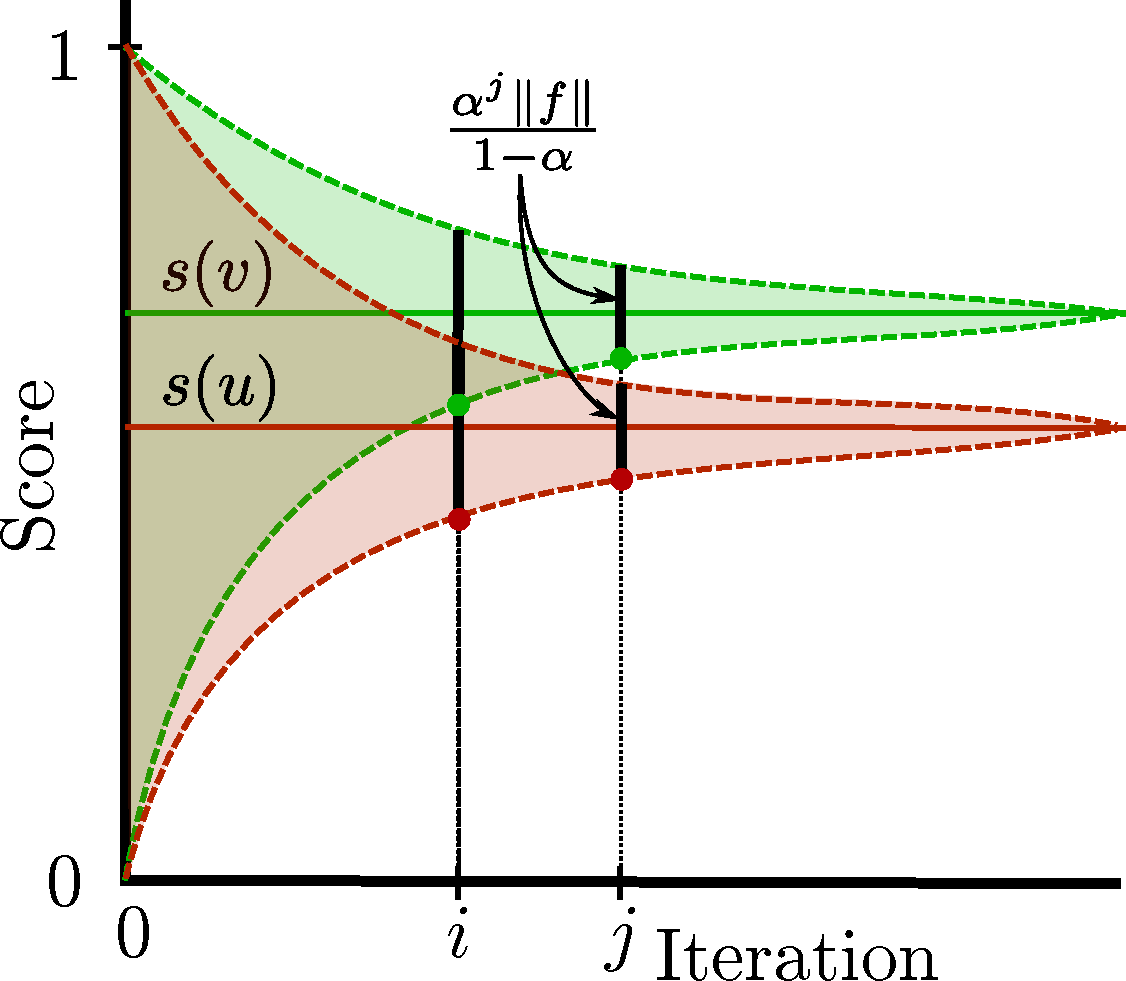
\includegraphics[width=0.4\textwidth]{figs/sink-source-squeeze-score-lb-ub-node-u-and-v-iteration-j.pdf}
    \caption{Overview of \SSS upper and lower bound comparison.}
    \label{fig:sinksource-squeeze-ub-lb}
\end{figure}

\subsubsection{\SSS proof}
TODO. See \cref{fig:sinksource-squeeze-ub-lb} for an example of the lower and upper bounds for two nodes at each iteration.

%\subsection{Lower Bound}
\par{Lower Bound}
%Each node always either increases or stays the same after each iteration. 
\begin{lemma}
\murali{State the lemma here.}
\end{lemma}

%\begin{proof}

From \cref{eq:sinksource-matrix-iteration} we have that $\vec{s}$ contains the final prediction scores for each node. We can efficiently approximate $\vec{s}$ by repeatedly iterating over \cref{eq:sinksource-matrix-iteration}, where at a given iteration $i$, 
\begin{equation}
%\label{eq:sinksource-matrix-iteration}
    \vec{s}^{(i+1)} = P\vec{s}^{(i)} + \vec{f}
\end{equation}

Below we first prove that each iteration produces a tighter lower bound vector (i.e., $\vec{s}^{(i+1)}$ closer to $\vec{s}$), and second, $\vec{s}^{(i)}$ finally converges to $\vec{s}$. 
We use the notation $\mathbf{x} \prec \mathbf{y}$ to signify that $\forall_i, x(i) \leq y(i)$.

(1) $\svec{0} = 0$, $\su{1} = f(u)$. Clearly $\svec{0} \prec \svec{1}$. Further, if $\svec{i-1} \prec \svec{i}$, then $\forall(u)$:

\begin{equation}
\su{i+1} - \su{i} = \alpha \sum\limits_{v\in{}N_u} p_{uv}\big[ \su{i} - \su{i-1}\big] \ge 0
\end{equation}

(2) Solving for \cref{eq:sinksource-matrix-iteration} gives us $\vec{s} = (I - \alpha{}P)^{-1}\vec{f}$. 
%Because $\lim_{i\to\infty}(\alpha{}P)^{i} = 0$, $(I - \alpha{}P)^{-1} = I + \alpha{}P + \alpha{}^2P^2 + \ldots \alpha{}^{\infty}P^{\infty} = \sum\limits_{j=0}^{\infty}(\alpha{}P)^j$ which was first shown in XX.
Because $\lim_{i\to\infty}(\alpha{}P)^{i} = 0$, $(I - \alpha{}P)^{-1} = \sum\limits_{j=0}^{\infty}(\alpha{}P)^j$ which was first shown in XX. \jeff{Why is this true? The limit to infinity doesn't seem to imply the second half.} Therefore we have that after every iteration, $\vec{s}^{i}$ is getting closer to $\vec{s}$.

\begin{equation}
\vec{s}^{(i)} \ = \ \sum\limits_{j=0}^{i}(\alpha{}P)^j \vec{f} \ \le \ \sum\limits_{j=0}^{\infty}(\alpha{}P)^j \vec{f} = \vec{s}
\end{equation}

Suppose $\svec{i} \prec \mathbf{s}$, then 
\begin{equation}
\su{i+1} \ \le \ \alpha \sum\limits_{v \in{} N_u} p_{uv}s(v) + f(u) \ = \ s(u)
\end{equation}
%\end{proof}

\par{Upper Bound}
\murali{Add an observation that states that $\|Ps\| \leq \|P\| \|s\|$.}

\begin{lemma}
For every node $u \in V$ and for every $i\geq 1$, $s(u) \ \le \ \su{i} + \frac{\alpha^i\|\mathbf{f}\|}{(1-\alpha)}$
\end{lemma}

Here, $\|\mathbf{x}\| = \|\mathbf{x}\|_{\infty} = \max\{|x_1|, \ldots |x_n|\}$. 
In the case of a matrix, $\|A\| = \|A\|_{\infty} = \max\limits_{i}\sum\limits_{j=0}^{n}a_{ij}$. 
Note that $\|P\| = 1$.

\textit{Proof}. $\forall i > 0$, 
\begin{align}
\svec{i+1} - \svec{i} \     &=   \ \alpha{}P(\svec{i} - \svec{i-1}) \\
\|\svec{i+1} - \svec{i}\| \ &\le \ \|\alpha{}P(\svec{i} - \svec{i-1})\| \\
                          \ &\le \ \|\alpha{}P\| \cdot \|\svec{i} - \svec{i-1}\| \\
                          \ &\le \ \alpha{} \|\svec{i} - \svec{i-1}\|
\end{align}

Repeatedly applying the above inequality gives us the following. 
\begin{equation}
\|\svec{i+1} - \svec{i}\| \ \le \ \alpha^{i} \|\svec{1} - \svec{0}\| = \alpha^{i}\|\mathbf{f}\|
\end{equation}

Now we need to account for the rest of the iterations up to $\infty$. 
We're effectively asking what is the greatest amount of score this node could accumulate in the following iterations? $\forall_m > i$
\begin{align}
\|\svec{m} - \svec{i}\| \ 
&=   \ \| \sum_{j=i}^{m-1}(\svec{j+1} - \svec{j}) \| \\
&\le \ \sum_{j=i}^{m-1}\| \svec{j+1} - \svec{j} \| \\
&\le \ \sum_{j=i}^{m-1} \alpha^{j}\|\mathbf{f}\| \\
&\le \ \alpha^i\|\mathbf{f}\| \sum_{j=0}^{m-i-1} \alpha^{j} \\
&\le \ \alpha^i\|\mathbf{f}\| \Big( \frac{1 - \alpha^{m-i}}{1 - \alpha} \Big) \\
\intertext{As $m\to\infty$, we have} 
\|\svec{m} - \svec{i}\| \ &\le \frac{\alpha^i\|\mathbf{f}\|}{(1-\alpha)}
\end{align}

\murali{The last statement is not enough. We have to prove that as $m \to\infty$, $\svec{m} \to \svec{}$.}

\murali{We also need to show that the upper bound improves as we change $i$ to $i+1$, i.e., $\su{i} + \frac{\alpha^i\|\mathbf{f}\|}{(1-\alpha)} \geq \su{i+1} + \frac{\alpha^{i+1}\|\mathbf{f}\|}{(1-\alpha)}$. In other words $\su{i+1} - \su{i} \leq \frac{(\alpha^i - \alpha^{i-1})\|\mathbf{f}\|}{1-\alpha} = \alpha^i \|\mathbf{f}\|$, which is true. }

There may be rare cases where a group of nodes have the same upper and lower bound, yet whose relative ordering with all other nodes is fixed. In these cases, we simply give them the same ranking as we have no way to distinguish how to order them in relation to each other. 

\subsection{Proof for $\alpha$}
\subsection{Proof for hierarchy consistent predictions}

A potential problem for methods which make term-based predictions is that they may not be consistent with parent-child relationships in the hierarchy. For example, if a GO term $t_i$ is a child of $t_j$, then if a method predicts a gene $g$ to be annotated with $t_i$ yet not to $t_j$, it would be inconsistent with the ontology. 
%in order to be consistent with the hierarchy, it must also predict $g$ to be annotated with $t_2$. 
In this section we provide a proof for \sinksource and \genemania that all predictions are hierarchically consistent.
%Specifically 

Let $s_i(u,k)$ be the score of node $u$ after $k$ iterations of \sinksource for a given term $t_i$. 
In order to give hierarchically consistent predictions, $s_i(u,k)$ must be $\leq s_j(u,k)$ at each iteration $k$, meaning for a given parent-child term pair, the prediction score of a gene for the parent term must always be equal to or greater than the score for the child term.
%meaning the prediction score of $u$ after $k$ iterations for $t_2$ must be $\leq$ the score of $u$ after $k$ iterations for $t_2$. \jeff{don't repeat, summarize here}

\begin{theorem}
For every parent $t_j$ and child $t_i$ term pair, node $u \in V$, and iteration $k$, $s_i(u,k) \leq s_j(u,k)$
\end{theorem}

First, we show the relationships between positive and negative examples for $t_i$ and $t_j$, then use them to prove the scores only either increase or stay the same when for a given node as we make predictions for terms higher in the hierarchy. 
According to our definition of negative examples (see \cref{sec:pos-neg-unk-examples}), all genes directly annotated with a term other than $t_i$ its ancestors will be considered a negative example for $t_i$. 
Let $V^+(t_i)$, $V^-(t_i)$, and $V^0(t_i)$ be the sets of positive, negative and unknown example for term $t_i$.  %\jeff{by def.} 
All positive, negative and unknown examples for $t_i$ and $t_j$ would be the same, except in the following two observations.
%The differences of positive, negative, and unknown examples from $t_i$ to $t_j$ are encompassed in the following three observations.
\begin{enumerate}[i.]
    \item $V^+(t_i) \subseteq V^+(t_j)$ and $V^-(t_i) \supseteq V^-(t_j)$. Genes directly annotated to siblings of $t_i$ and their descendants, would be positive examples for $t_2$, yet negative examples for $t_i$.
    %\item $V^+(t_i) \subseteq V^+(t_j)$. Genes directly annotated to siblings of $t_i$ and their descendants, would be positive examples for $t_2$, yet negative examples for $t_i$
    %\item $V^-(t_i) \supseteq V^-(t_j)$. Same reasoning as above.
    \item $V^0(t_i) \subseteq V^0(t_j)$. Genes annotated directly to $t_j$ would be positive examples for $t_j$ and unknown examples for $t_i$.
\end{enumerate}
%We observe that , $V^-(t_i) \supseteq V^-(t_j)$, and $V^0(t_i) \subseteq V^0(t_j)$ as  would be genes which are directly annotated to $t_j$ and its descendent terms, excluding $t_i$ and its descendants. %which would be positive examples for both $t_1$ and $t_2$. 
%Let $D(t_i)$ include $t_i$ and its descendants in a given hierarchy.
%sibling terms of $t_1$, or other 
%Genes directly annotated to descendants of $t_j$, excluding $t_1$ and its descendants, would be positive examples for $t_2$, yet negative examples for $t_1$. 
%$U(t_2) = U(t_1) - P(t_2)$. 
Below we prove $s_1(u,k) \leq s_2(u,k)$ at each iteration $k$ by induction.

\paragraph{\sinksource.}
Base case: $s_1(u,1) \leq s_2(u,1)$.
\begin{align}
    s_i(u,1) &= \alpha \sum_{\mathclap{v \in N^0_i(u)}} p_{uv}s_i(v,0)  + f_i(u) = 0 + f_i(u) \\
    s_j(u,1) &= \alpha \sum_{\mathclap{v \in N^0_j(u)}} p_{uv}s_j(v,0)  + f_j(u) = 0 + f_j(u)
\end{align}
where $N^0_i(u)$ is the neighbors of $u$ in $V^0$ for $t_i$.
%\shortintertext{Because $P(t_1) \subseteq P(t_2)$ and $N(t_1) \supseteq N(t_2)$ the 
Because of the observation that $V^+(t_i) \subseteq V^+(t_j)$ and $V^-(t_i) \supseteq V^-(t_j)$, $f_i(u)$ would have less positive neighbors and more negative neighbors than $f_j(u)$, meaning
\begin{align}
      f_i(u) &\leq f_j(u) \label{eq:fi_leq_fj}%\\
%\shortintertext{thus proving}
%    s_1(u,1) &\leq s_2(u,1)
%    \alpha\sum_{\mathclap{v \in N^{+}_{1}(u)}} P_{uv}(1) &\leq \alpha\sum_{\mathclap{v \in N^{+}_{2}(u)}} P_{uv}(1)
\end{align}
%where $f_i(u) = \alpha \sum_{v \in N^{+}_{i}(u)} P_{uv}(1)$ is the amount of fixed score coming from neighbors of $u$ in $V^+$ for term $t_i$. Negative examples are fixed at $0$ and therefore do not contribute to the score. \jeff{move this above}
%Because $V^+(t_1) \subseteq V^+(t_2)$ and $V^-(t_1) \supseteq V^-(t_2)$, meaning $t_2$ has more positive and less negative examples than $t_1$, \cref{eq:f1_leq_f2} holds.
Suppose that $s_i(u,k-1) \leq s_j(u,k-1)$.
By the inductive hypothesis, we show $s_i(u,k) \leq s_j(u,k)$ as follows
\begin{align}
    s_i(u,k) &= \alpha \sum_{\mathclap{v \in N^0_i(u)}} p_{uv}s_i(v,k-1) + f_i(u)  \\
          &\leq \alpha \sum_{\mathclap{v \in N^0_i(u)}} p_{uv}s_i(v,k-1) + f_j(u) \text{, \cref{eq:fi_leq_fj}} \\
          &\leq \alpha \sum_{\mathclap{v \in N^0_j(u)}} p_{uv}s_j(v,k-1) + f_j(u) \text{, by the inductive hypothesis} \\
             &= s_j(u,k)
\end{align}

thus completing the proof.
%The above reasoning holds true for all ancestors of $t_i$, thus ensuring that for genes, all predictions are hierarchically consistent.


\subsection{Datasets}
\label{sec:datasets}

\subsubsection{Sequence Similarity Network}
\label{sec:ssn}
We created a network based upon sequence similarity of the putative proteomes of 19 clinically-relevant pathogenic bacteria.
We downloaded sequences and GO annotations from UniProt~\cite{uniprot-consortium-uniprot-nar-2017}.
In instances where multiple UniProt reference strains were available for a pathogen, we chose the reference proteome with the largest number of GO annotations.
We performed an all-vs-all BLASTP and processed the results by 
%removing \evals $\geq$ 0.1,
%(ii) deleting matches where the length of the sequences differed by $>$ 20\%, % effusion has a better description for this processing step
retaining the weaker score for all reciprocated matches, removing self-comparisons, and using the absolute value of the base-10 logarithm of the \eval as the edge weight. 
For edges where the \eval was 0, we assigned a score of 180 which is the -log$_{10}$ of the smallest non-zero \eval observed (rounded).
For networks where we used an \eval cutoff $> 1$, we added log$_{10}$ of the cutoff to the edge scores to ensure all edges had a positive score.
We tested various \eval cutoffs from \e{-25} to 50 (see Table \ref{tab:net-sizes} for the number of nodes and edges).
%The resulting network (referred to as \SSN) contained 60K proteins connected by 2.5M edges.

\subsubsection{STRING Networks}
\label{sec:string}
We integrated species-specific STRING functional association networks for 14 of the 19 bacterial species where ID mapping from UniProt was available (STRING v10.5, downloaded on 2017.09.18)~\cite{szklarczyk-mering-string-v10.5-nar-2017}.
% We recognize that using a more sophisticated method such as that used by INGA of mapping using BLAST would increase our coverage, however, the ID mapping worked well enough for our evaluations here.
STRING assigns edge weights based on evidence of association including physical binding, gene expression, orthology mapping and more. 
Specifically, we utilized six STRING networks: neighborhood, fusion, cooccurence, coexpression, experimental, and database.
% move this point to discussion or results
We found including all available networks did not improve the quality of results above the six core networks (results not shown).
%We chose not to include the networks with evidence transferred based on orthology to ensure that when performing an evaluation for a given species, we did not transfer evidence from 
%Combining those 50K nodes and 2.4M associations with the SeqSim network yielded a network (referred to as Integrated) with 70K nodes and 5M edges.
We also tested various STRING cutoffs including 150, 400 and 700 (low, medium and high stringency) cutoffs (see Table \ref{tab:net-sizes} for network sizes). 
%\murali{Move to supplement; you can refer to this table in the main text.}



\subsubsection{Gene Ontology Annotations}
\label{sec:goa}
We obtained GO~\cite{gene-ontology-consortium-go-expansion-nar-2017} annotations for these bacteria from the UniProt-GOA database (``goa\_uniprot\_all.gaf.gz'' Downloaded on 2017.09.18).
% ftp://ftp.ebi.ac.uk/pub/databases/GO/goa/UNIPROT/goa_uniprot_all.gaf.gz
%We considered two subsets of annotations: (a) EXP: only based on experimental evidence codes and (b) non-IEA: EXP codes as well as codes based on curator verified sequence similarity annotations. A total of 154 molecular function (MF) and 453 biological process (BP) GO terms were annotated to at least 100 proteins with a non-IEA evidence code. 13K proteins had at least 1 non-IEA annotation, and 6K had at least 1 EXP annotation. For each GO term, we treated every gene that was not annotated to any ancestor or to any descendant term as a negative example.
%
% evidence codes
We considered three sets of evidence codes: (i) Experimental as well as those used in CAFA (EXPC): EXP, IDA, IPI, IMP, IGI, IEP, TAS, IC; (ii) Computational Analysis (COMP): ISS, ISO, ISA, ISM, IGC, IBA, IBD, IKR, IRD, RCA; and (iii) Electronic Analysis (ELEC): IEA.
A total of 319 biological process (BP) and 117 molecular function (MF) GO terms were annotated to at least 50 proteins with an EXPC evidence code.
% We recognize there is a potential circularity issue where the 

%\subsubsection{Selecting Bacterial Species}
%As a proof-of-concept, we selected 19 clinically relevant bacteria. 
%%We also sought to scale-up to include many more bacterial species. 
%To scale-up to include many more organisms, we simply selected the top 200 bacterial species with the most EXPC or COMP annotations which ranged from six to 16,685 (\textit{Gluconobacter oxydans} and \textit{Escheria coli} respectively).

\subsubsection{Positive, Negative, and Unknown Examples}
\label{sec:pos-neg-unk-examples}
We say that $g$ is \emph{directly} annotated to $t$ if this annotation appears in the annotations (GAF) file. For a given GO term $t$, we defined a gene $g$ as 
\begin{enumerate}[(a)]
    \item a \emph{positive example} if $g$ was directly annotated to $t$ or to a descendant of $t$ in the GO DAG, 
    \item a \emph{negative example} if $g$ was not directly annotated to $t$ or to an ancestor or descendant of $t$ in the GO DAG, but also had at least one other annotation, and 
    \item an \emph{unknown example} otherwise.
\end{enumerate}
This approach is commonly used in the literature~\cite{mostafavi-morris-genemania-gb-2008}.
%  and a given set of positive evidence codes $EC$  % with an evidence code in $EC$
In several analyses, we restricted our attention to a specific set of evidence codes, e.g., experimental ones. In such a situation, we discarded all direct annotations with other evidence codes before computing the different sets of examples.
%For example, if we used EXPC annotations to define positive examples, we also used EXPC annotations to define negative examples.
%Additionally, if $g$ was assigned as a negative example for $t$ but has an electronic annotation  (i.e., IEA), we removed it as a negative example for $t$.
In addition, if a gene $g$ satisfied the conditions to be a negative examples for a term $t$ but also had an electronic annotation (i.e., evidence code IEA) to $t$, we considered $g$ to be an unknown example for $t$.
%Improving our selection of negative examples would improve the performance at various 

We utilized these three sets of examples in different aspects of this work: (a) for integrating multiple networks, (b) for algorithms which use negatives examples (\sinksource and \genemania), and (c) for defining false positives when evaluating. \murali{Add section numbers.}


\subsection{Network Integration}
\label{sec:network-integration}
%\jeff{probably shouldn't go under datasets}
We compared two kernel-based network integration methods.
\begin{description}
\item[1) \genemania-2008] \hfill \\
Mostafavi and Morris integrated multiple networks on a GO term-by-GO term basis using ridge regression~\cite{mostafavi-morris-genemania-gb-2008}. %Loosely, for a given GO term, the networks are given a score based on how well the edge weights match the positives vs. the negatives. The networks are then combined by taking the sum of the edge weights in each network, multiplied by its score.
Given $m$ \FLN{}s encoded as matrices $W_{1},...,W_{m}$, they combined the networks using:

\begin{equation*}
    W^{comb} = \sum\limits_{i=0}^{m} \mu_{i}W_{i}
\end{equation*}

where the network weights, $\mu = [\mu_1, \mu_2, ..., \mu_m]$, are assigned by solving a constrained linear regression problem for a specific prediction task. 
\jeff{Include the equation here}.

\item[2) SWSN] \hfill \\
%Mostafavi and Morris later improved their original method by computing optimal weights for multiple related GO terms simultaneously~\cite{mostafavi-morris-fast-integration-bioinfo-2010}.
Youngs \etal followed a similar framework where they compute an optimal weight for each network, however they extend the method to be able to compute the weights for multiple related GO terms simultaneously using specific negative examples (Simultaneous Weights with Specific Negatives, SWSN)~\cite{youngs-bonneau-better-negatives-pfp-bioinfo-2013}. 
They found that fitting the weights to all GO terms in a particular hierarchy (i.e., BP or MF) worked better than any other grouping of functions. 
We also grouped GO terms by hierarchy to compute the optimal weights for our networks.
%once for a given set of GO terms with an approach similar to the previous method in the case of individual GO terms~\cite{youngs-bonneau-better-negatives-pfp-bioinfo-2013}. While there are many ways to combine the GO terms, we only used the sets of all GO terms in a given hierarchy (BP or MF) which they found performed the best.

\end{description}
% discussion section?
% In our experiments, we found that the in
Interestingly, in our experiments we found that using the original integration method proposed by Mostafavi \etal resulted in better performance than the SWSN method for \sinksource and \genemania, especially for MF GO terms (results not shown).
For \birgrank, we were limited to the SWSN method as for a given protein, all GO term predictions (for a given hierarchy) are made simultaneously.


\subsection{Evaluation}
\label{sec:evaluation}
\subsubsection{Leave-One-Species-Out Evaluation}
We evaluated each algorithm using a leave-one-species-out validation method where we iteratively leave out the annotations of all proteins of a single species, and use the annotations of the other 18 species to make predictions for the left out species (see \fig \ref{fig:leave-one-species-out}). This evaluation is meant to test our ability to make functional predictions for the genome of a newly sequenced species where none of the proteins have any previous annotations. 

\begin{figure}[htb]
    \centering
    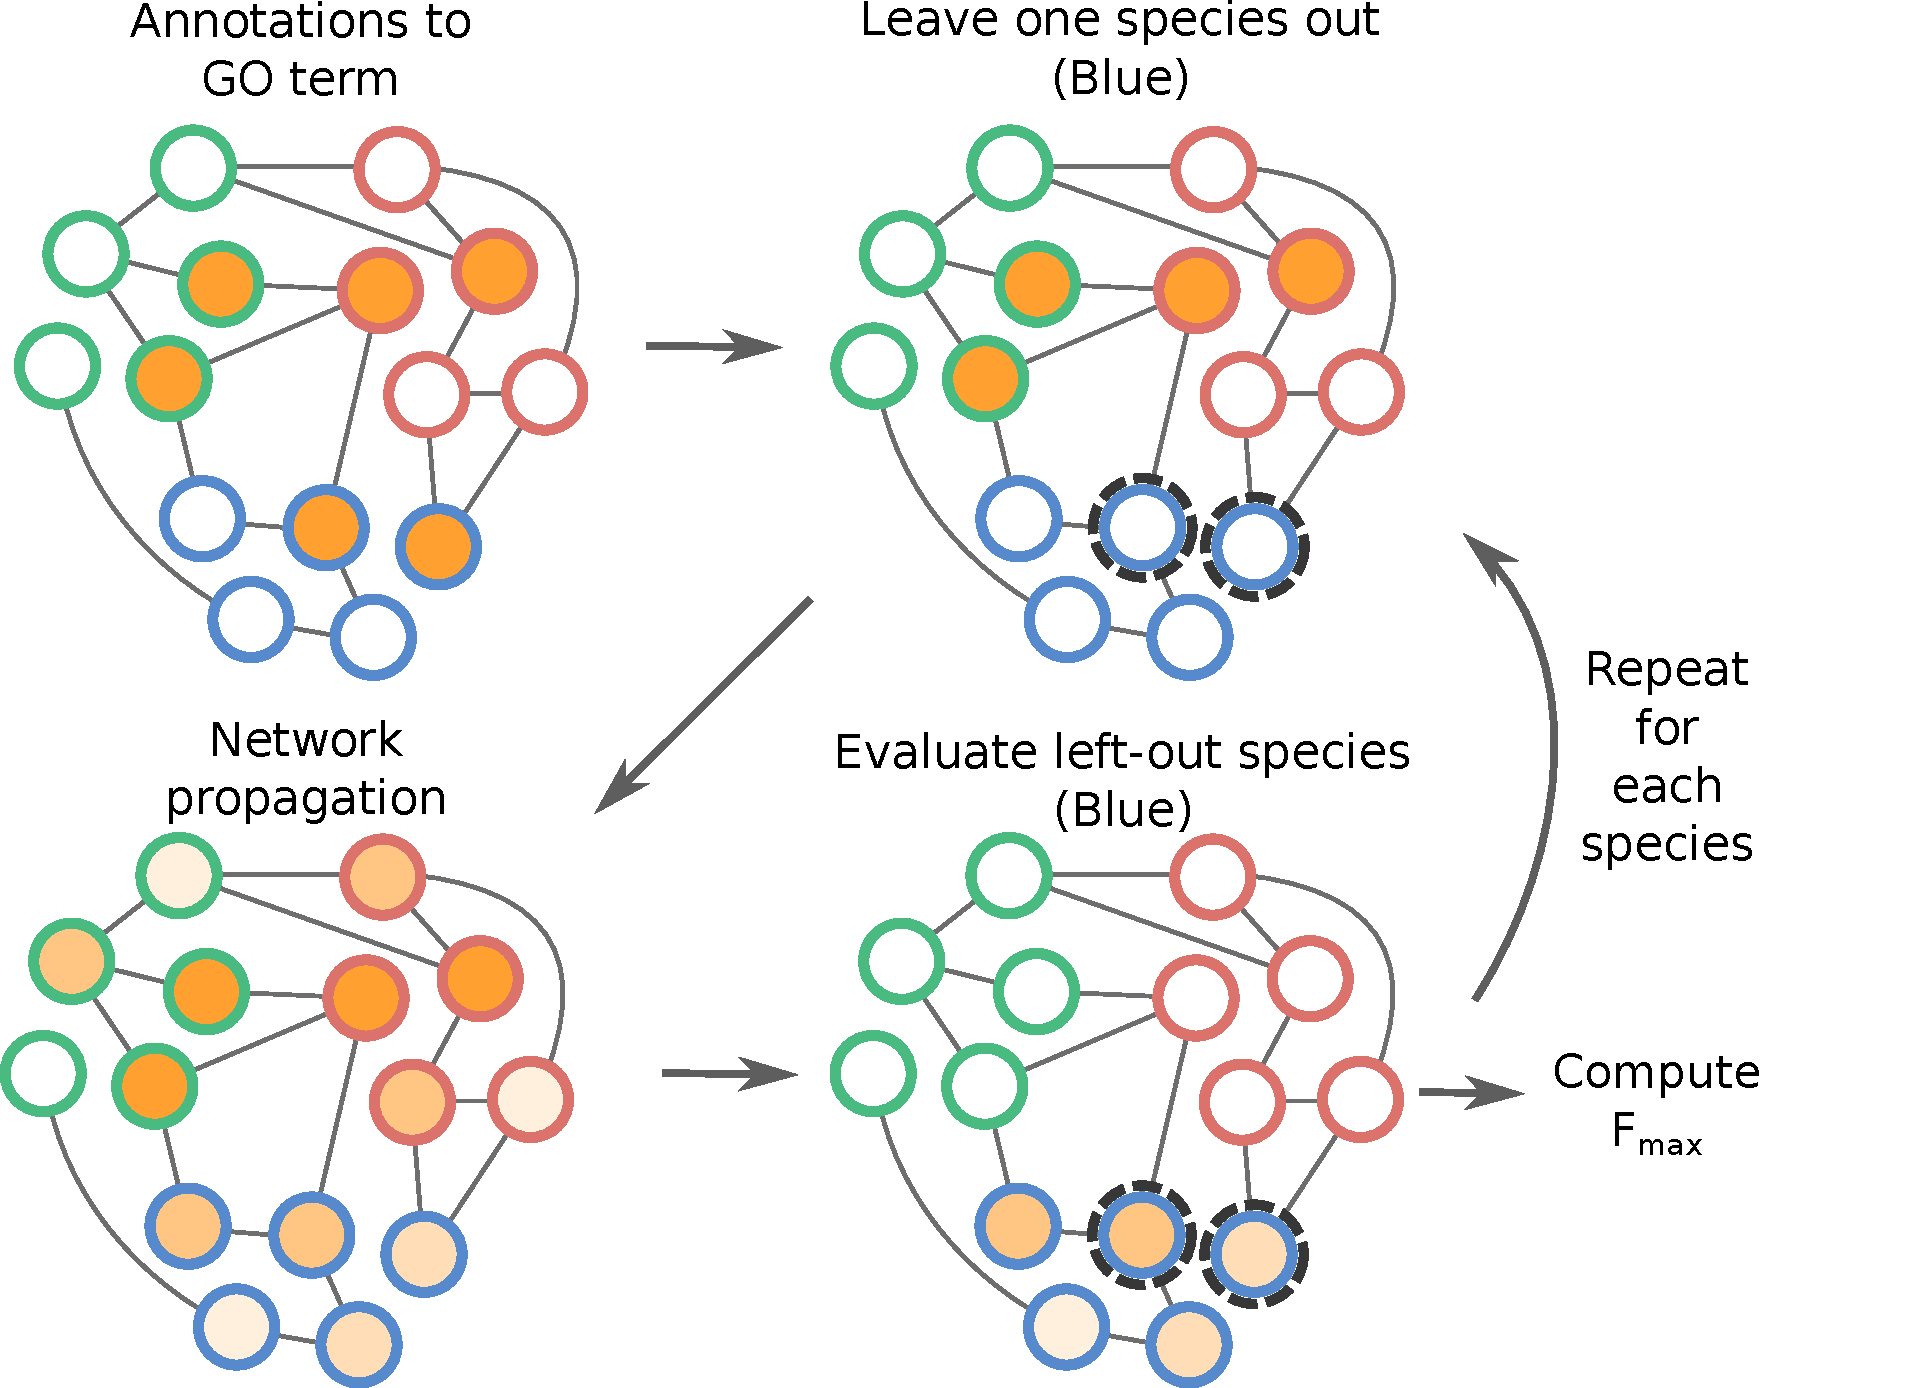
\includegraphics[width=0.5\textwidth]{figs/leave-one-species-out.pdf}
    \caption{Overview of the leave-one-species-out evaluation. The picture represents a \SSN where the border colors represent a species. The orange nodes represent proteins annotated with a given GO term (top left). All annotations are left out for a given species (top left) and evaluated how well they can be recovered (bottom right) by propagating the annotations from the known proteins to the nearby unknown proteins (bottom left). This process is repeated for all GO terms and all species.}
    \label{fig:leave-one-species-out}
\end{figure}

We chose to first evaluate using only the experimentally-based annotations. 
When evaluating predictions for a given left-out species, true positives and false positives are calculated from the positive and negative examples of that species.
%However, as only a few species have a decent amount of experimentally-based annotations, we also expanded our evaluation to include annotations with either an experimental, or computational evidence codes as defined above. 
%A total of 9 species have at least one GO term for which 10 or more proteins are annotated. 

We used the \fmax value to compare algorithms, as it is used in the critical assessment of functional annotation (CAFA) challenge. 
%\subsubsection{Temporal Holdout}
%June 2016 - September 2017


\section{Results}


We investigate and discuss our results for the Biological Process (BP) category in the main text. We include the results for the evaluation of Molecular Function (MF) in the supplementary material. \murali{Rather than simply put the MF results in the supplement, we will have to refer to them in meaningful ways in the main text.}

We evaluated each method using leave-one-species-out (LOSO) validation with 19 bacterial species where we mimicked the challenge of making large-scale functional predictions for the genome of a newly-sequenced species %where none of the genes have any previous annotations. 
that has no previous annotations.
We constructed a multi-species network, left out the annotations of all genes for each species in turn, and used the annotations of the other 18 organisms to make predictions for the left-out species (see \cref{fig:leave-one-species-out}). 
First, we tested the trade-off between accuracy and speed for \sinksource by varying either $\alpha$ or the number of iterations, \murali{We have to describe the other sections as well.}
and later use the selected parameters as we scale-up to 200 bacterial species.
%We then evaluated three network propagation methods---\sinksource, \genemania and \birgrank---against the baseline \localplus method.
%Then we analyze the compare the effect of choosing different BLAST \eval cutoffs and STRING cutoffs to build the multi-species network


\subsection{Trade-off between Accuracy and Speed}
\label{sec:tradeoff-accuracy-speed}

%\murali{State the goals of the experiment (We first ...), then the way you performed the experiment, then refer to the figure and describe, the results.}
By design, \sinksource converges faster, i.e., with a smaller number of iterations as we decrease the parameter $\alpha$  \murali{Refer to lemma in the supplement.} Additionally, for a fixed $\alpha$, \sinksource terminates faster as we decrease the number of iterations. Therefore, we sought to test the trade-off between accuracy and speed by varying either $\alpha$ or the number of iterations before we stopped \sinksource. 
%\murali{Where have you defined ``stopping criteria'' before? I modified the sentence since it was potentially confusing as written. It could mean that $\alpha$ controls accuracy and the other criterion controls speed. But that is not what you intended to say, is it?}


First, we ran \sinksource for eight different values of $\alpha$, namely, 1, 0.99, 0.95, 0.9, 0.8, 0.7, 0.6, and 0.5. 
%\murali{You are in the middle of describing the setup for these experiments. Don't mention results here. Mention them in the next para. "which is double the number of iterations required to fix the rankings for $\alpha = 0.9$, and which resulted in an average $\epsilon$ of \e{-4}" \jeff{need to show this data in the supp.}.} 
% no longer five-fold cross-validation
For each value, we performed the \loso evaluation for each of the 19 bacterial species using the \SSN (\eval $\leq 0.1$) integrated with STRING and only annotations with experimental evidence codes. We considered 319 biological process GO terms, each with at least 50 annotations summed over all 19 organisms. For each "left-out" species, we limited the evaluation to the GO terms with at least 10 annotations in that species.
For values of $\alpha < 1$, we executed \sinksource to convergence, i.e., we used as many iterations as needed to fix the relative rankings of the positive and negative examples in the left-out species, ignoring the bounds for the other examples in our test for fixed ordering.
%executed \sinksource to convergence, i.e., until every left-out positive or negative node had a distinct upper and lower bound. We called the resulting ranking of nodes as the "fixed ordering." \murali{What do we do about ties? Where do we discuss this issue?} \jeff{If they're fixed compared to all other nodes, we fix their ranking as well. I made a note of this in the methods.}
For $\alpha = 1.0$, the upper bound on the node score we can prove is trivially equal to unity in each iteration. 
%\murali{"Squeeze upper bound": This phrase does not sound good. You have to refer to a lemma or a theorem or "our upper bound". I also don't want Squeeze to appear in the paper anywhere but the place where we prove our theory.} 
Therefore, we stopped \sinksource after 1000 iterations. 

We explored the effect of varying $\alpha$ on the accuracy of \sinksource by comparing the resulting distributions of \fmax values (\cref{fig:sinksource-speed-vs-accuracy}a). 
The median \fmax value did decrease gradually as we decreased $\alpha$. 
For $\alpha \leq 0.8$, we observed a statistically significant difference compared to $\alpha = 1.0$ (uncorrected \pval $\leq$ 0.1).
However, we did not observe a significant difference between the distributions for $\alpha = 1.0$, and $\alpha = 0.99$, $\alpha = 0.95$, and $\alpha = 0.9$, with the median of differences between the \fmax for each GO term of 0.0, 0.002, and 0.005 respectively (rank-sum test, uncorrected \pval 0.45, 0.28, and 0.17 respectively).
%However, we did not observe a statistically-significant difference between the distributions for $\alpha = 1.0$ and $\alpha = 0.8$ (rank-sum test, uncorrected \pval = 0.08).
%We note that the rank-sum test could lead to overly-optimistic \pval{}s as GO terms are not fully independent from each other.  \murali{Use brackets only for small phrases and not for multiple sentences. More importantly, why mention over optimism here when the \pval{}s are not significant? Over-optimism is an issue only if the p-values are small.}
%We recognize the choice of $\alpha$ for \sinksource is somewhat arbitrary and depends on specific use cases. In our experiments, for $\alpha < 0.8$, the rank-sum \pval fell below 0.05, 
We chose $\alpha = 0.95$ for subsequent analyses.  

% # of iterations
Next, we considered varying the number of iterations for which we ran \sinksource. We first executed \sinksource to convergence, i.e., the node orderings were fixed.
We then re-executed \sinksource and for each $i > 0$, we compared how similar the node ranking after iteration $i$ was to the fixed ordering using \ktau, a measure of rank correlation. Given two different rankings of the nodes, this measure counts the fraction of node pairs that are not inverted, i.e., the fraction of node pairs $u$ and $v$ such that $u$ appears before $v$ in both rankings or vice-versa. Thus, the closer $\tau$ is to unity, the more similar are the two rankings. For each GO term, we recorded the number of iterations needed to reach a correlation of 0.9, 0.95, 0.99, and 1.0 (\cref{fig:sinksource-speed-vs-accuracy}b). 
%, and the largest stretch of nodes with overlapping upper or lower bounds. 
%The \ktau statistic will advise us as to how many iterations are needed to approximate the fixed ranking.
The median number of iterations required to fix the node ordering was 359. Interestingly, we observed that \sinksource computed this ranking sooner with a median of 170 iterations (see \cref{fig:sinksource-speed-vs-accuracy}b, \ktau = 1.0); subsequent iterations did not change the ordering but were necessary to guarantee that it would not be modified by more iterations. 
% precision problem:
% This is partially due to the limited 80-bit precision of numpy.  At about 200 iterations, the maximum precision for node scores is reached, and the maximum difference of node scores from one iteration to the next drops to 0 meaning the node scores cannot be approximated any better. Squeeze maintains a single value $x$ to compute the upper bound for all nodes which is the lower bound plus $x$. The upper bound value $x$ does not require many digits to compute, and can be stored with leading zeros meaning it does not suffer from loss of precision allowing us to better approximate it the upper bounds. After 400 iterations, the upper-bound is small enough to ensure the nodes have distinct upper and lower bounds. As we are primarily concerned with the values of the first few digits and not the full precision, we decided not to bother computing the full precision on a platform such as matlab 
Even more strikingly, after a median of 29 and 18 iterations, \ktau was already as high as 0.95 and 0.90, respectively.
These results suggested that while about 360 iterations may be required to provably fix the rankings of the left-out positive and negative nodes, reducing the number of iterations by a factor of 20 does not have a material impact of the relative orderings of most of the positive and negative node pairs. Moreover, fewer iterations may not be deleterious to the accuracy of \sinksource during evaluation.

To test this hypothesis, we fixed $\alpha = 0.95$, ran \sinksource for eight different number of iterations (400, 200, 50, 20, 10, 5, 2, and 1, and recorded the
% node rankings \murali{Where are the results for node ranking?} 
%\jeff{For 10 iterations, the median \ktau is about 0.85, 5 is 0.79, 3 is 0.7 and 1 is 0.17} and 
\fmax values after \loso validation (\cref{fig:sinksource-speed-vs-accuracy}c). The \fmax distribution for 400 iterations was statistically indistinguishable from the distribution for each of the next four largest number of iterations (200, 50, 20, and 10, rank-sum test, \pval $\geq 0.25$).
%, with medians of \fmax differences equal to 0 for $\geq 20$ iterations, and 0.004 comparing 400 to 10 iterations.
We concluded that decreasing the number of iterations by as large a factor as 40 did not affect the overall distribution of \loso performance. 
% running time
%The running time improved by a factor of 50 (331 minutes for \sinksource with $\alpha = 1.0$ for 1000 iterations vs. 6.6 minutes for 20 iterations with $\alpha = 0.8$, \fig \ref{fig:sinksource-speed-vs-accuracy}d). 
The running time improved by a factor of 50 (126.6 minutes for \sinksource with $\alpha = 1.0$ for 1000 iterations vs. 2.53 minutes for 20 iterations with $\alpha = 0.95$, \cref{fig:sinksource-speed-vs-accuracy}d). 
%\jeff{I need to re-run this with nothing else running on the machine to make sure they're accurate}
We chose to run \sinksource with $\alpha = 0.95$ and 20 iterations in all subsequent analyses for BP GO terms. 

We repeated the above process for all 117 MF GO terms with at least 50 annotations summed over all 19 organisms. We found $\alpha$ and the number of iterations to have a slightly larger effect on the \fmax with the median dropping more rapidly \jeff{(see figure X in supp TODO)}. 
\jeff{However, there is not a statistically significant difference for $\alpha \geq 0.8$,  possibly be due to the fact that there are fewer MF GO terms.}
For $\alpha = 0.95$, the median of \fmax differences compared to $\alpha = 1.0$ was 0.018 (rank-sum \pval 0.28). 
The \ktau reached 0.9 and 0.95 after 15 and 26 iterations respectively with a median of \fmax differences of 0 comparing 400 to 20 iterations (rank-sum \pval 0.38).
We chose to also use $\alpha = 0.95$ and 20 iterations for MF GO terms in subsequent analyses.

% additional analyses
%In the supplementary material, we compare how many iterations it takes to reach standard $\epsilon$ cutoffs as well as the distribution of \ktau at those cutoffs. 
%We also took into consideration how much of an effect number of iterations as well as the $\alpha$ parameter have on the results and find they do not have a significant effect (see \fig \ref{fig:sinksource-speed-vs-accuracy}a,c). 


% expc-rem-neg-comp-iea
\begin{figure}[H]
    \centering
    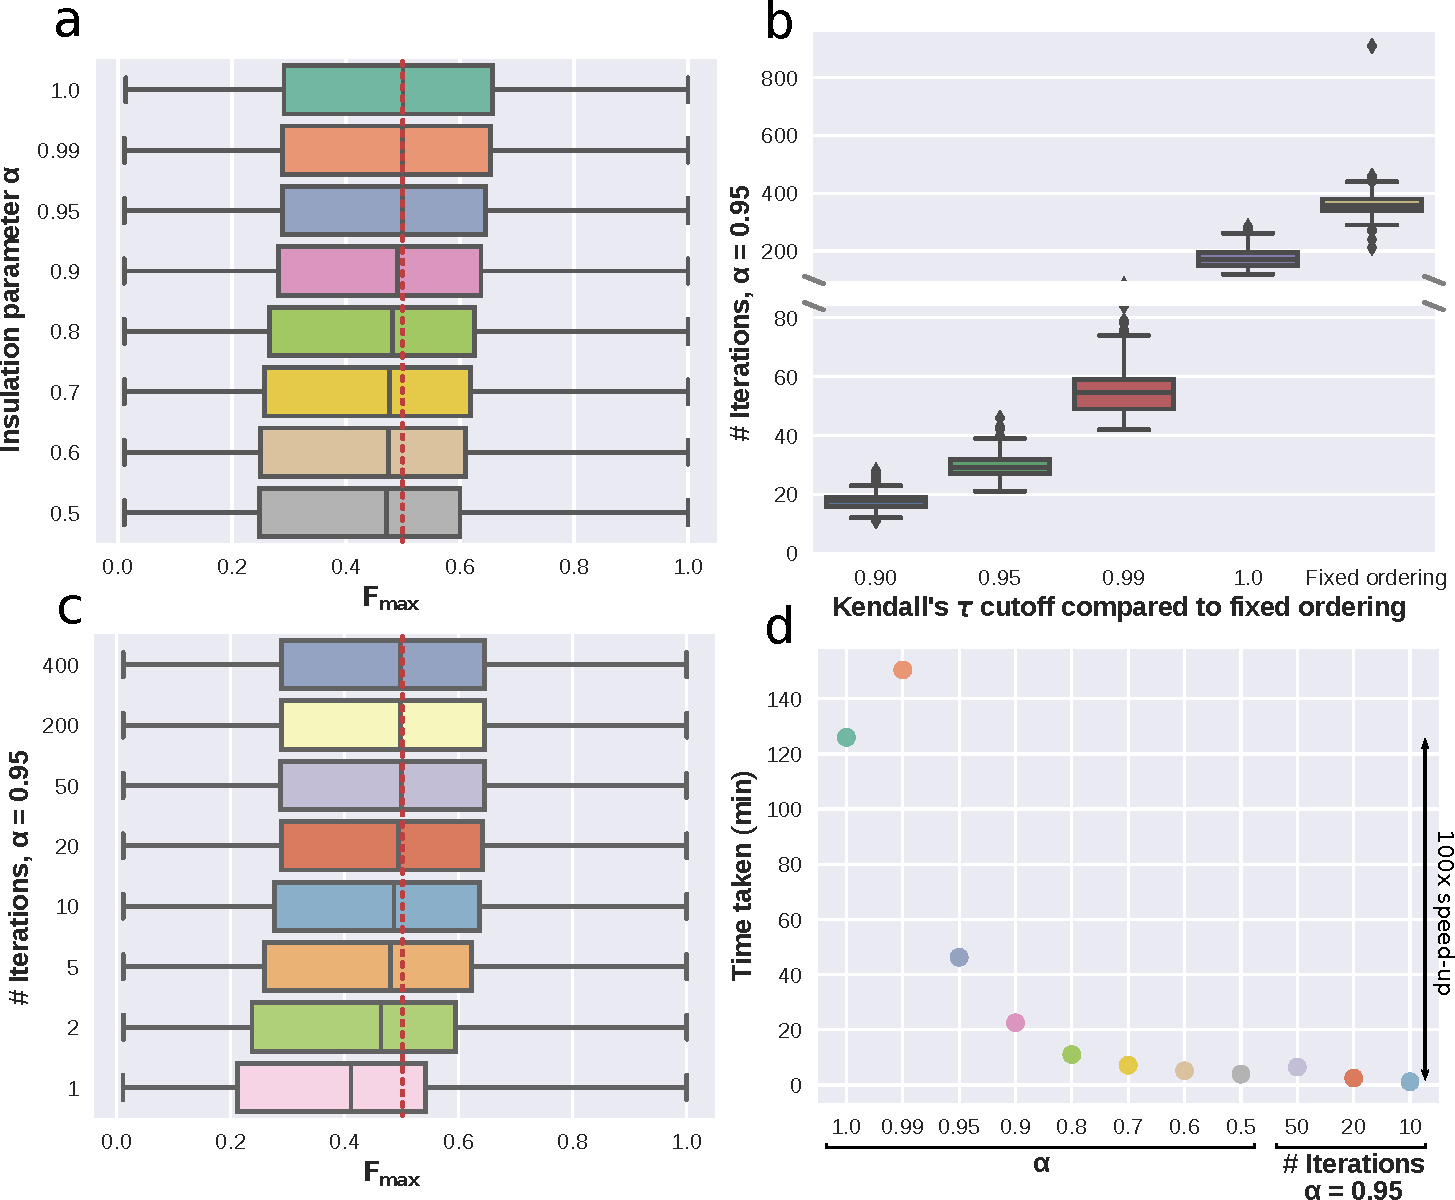
\includegraphics[width=\textwidth]{figs/fig1-2018_06-seq-sim-e0_1-string-expc-rem-neg-comp-iea-50-1000-bp-a0_95.pdf}
    \caption{Trade-off between accuracy and speed for \sinksource on the 19 bacterial species \SSN (\eval <= 0.1) with 319 BP GO terms ($\ge 50$ annotations) for the \loso evaluation. 
      %Performance is measured by computing the \fmax on a GO term by GO term basis. Here we used annotations of BP GO terms with experimental evidence codes
      (\textbf{a}) Variation of \fmax distributions with $\alpha$. The vertical red dotted line represents the median \fmax for $\alpha = 1.0$.
      (\textbf{b}) Number of iterations required to fix the rankings of the left-out positives and negatives, or to reach a specified value of \ktau in comparison to the fixed ranking.
      (\textbf{c}) Variation of \fmax distributions with the number of iterations ($\alpha=0.95$). The vertical red dotted line represents the median \fmax for $\alpha = 1.0$ in panel (a).
      (\textbf{d}) Total time taken by \sinksource (shown in a and b) while varying $\alpha$ or the number of iterations with $\alpha=0.95$. Colors are the same as in (\textbf{a}) and (\textbf{c}).
    }
    \label{fig:sinksource-speed-vs-accuracy}
\end{figure}

\subsection{Effect of BLAST \eval Cutoffs}
\label{sec:effect-eval-cutoffs}


Here, we studied the effect of using different \eval cutoffs to construct the sequence-similarity network, as this parameter can drastically change the size of the network (see Table \ref{tab:net-sizes}), with the largest \SSN containing over five million edges. 
%relatively high \evals can lead to spurious prediction results \jeff{TODO find citation}.
 

% evidence codes
In these evaluations, we first used annotations with at least one experimental evidence code. 
%for both making predictions, and evaluating the predictions.
%which is the standard set in CAFA~\cite{jiang-radivojac-cafa2-eval-function-prediction-gb-2016}.
As only a few species had a substantial number of experimentally-based annotations, we also expanded our evaluation to include annotations with either an experimental or computational evidence code, as well as all annotations regardless of evidence code (see \cref{sec:loso-results-expc-comp-iea}).

% BLAST cutoff makes a big difference for BP and MF
% network propagation still helps


When working with large networks, an initial approach may be to limit the number of edges using a stringent cutoff, and allow the propagation methods to make predictions using the edges with relatively high homology. 
%Such an approach is common when using a co-expression network \jeff{cite}.
Additionally, intuition would suggest that including many edges with relatively low homology would lead to more false positives \jeff{PFP and PhyloPFP used \evals up to 100. The BLAST webpage suggests a cutoff of \e{-6}, Effusion uses a cutoff of \e{-8}}. 

We tested cutoffs of \e{-25}, \e{-15}, \e{-6}, $0.1$, 5, 20 and 50 to evaluate at which cutoff we achieve the best performance.
We found that when we raised the \eval cutoff from \e{-25} to $0.1$, the median \fmax for each method increased by more than $0.1$ (rank-sum test \pval $4.2\times{}10^{-8}$, see \cref{fig:loso-results-exp}a,b).
Further raising the \eval cutoff past $0.1$ did not improve the median \fmax further (see Supplementary Text for results for \eval cutoffs of \e{-15} and \e{-6}, 5, 20, and 50).
We also observe that network propagation methods gain more of an advantage over \localplus for the more stringent \e{-25} cutoff than the 0.1 cutoff as expected, however we still see a marginal improvement at the 0.1 cutoff (rank-sum \pval = $3.5\times{}10^{-5}$ and $0.055$ respectively).

\begin{figure}[H]
    \centering
    %\jeff{figure placeholder}
    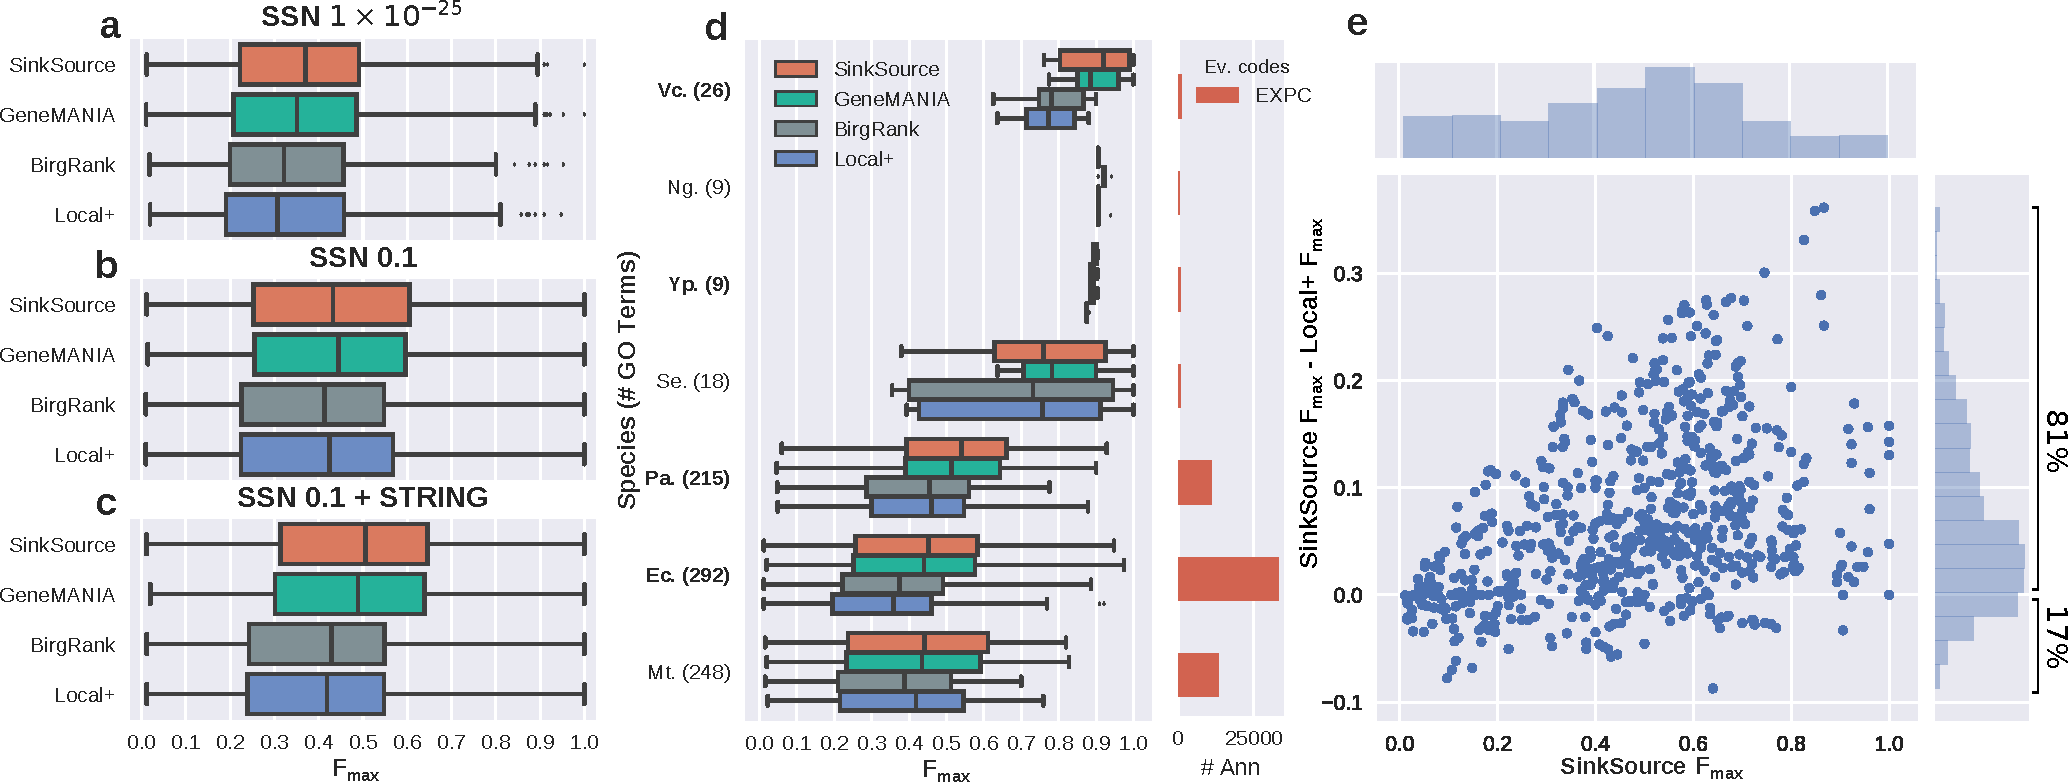
\includegraphics[width=\textwidth]{figs/fig2-expc-compare-eval-fmax-sinksource-localplus-bp-a0_95.pdf}
    \caption{
      Comparison of \fmax results for \loso evaluation across four algorithms and three networks.
      (\textbf{a}) \SSN (\eval $\le$ \e{-25}),
      (\textbf{b}) \SSN (\eval $\le$ 0.1),
      (\textbf{c},\textbf{d},\textbf{e}) \SSN (\eval $\le$ 0.1) integrated with STRING,
      (\textbf{d}) \loso results for individual species, sorted in decreasing order of median \fmax. The number of BP GO terms with $\ge$ 10 annotations appears in parentheses next to each species name.  The species name is in bold if the difference between the distributions for \sinksource and \localplus was statistically significant (rank-sum Bonferroni-corrected \pval $< 0.05$). \protect The right-hand side shows the number of GO term-annotation pairs with experimental evidence codes for each species.
    %315 total BP GO terms have at least 10 annotations in the left-out species. 
    Species names are abbreviated as follows:
    \textit{Escherichia coli K-12} (Ec),
    \textit{Mycobacterium tuberculosis} (Mt),
    \textit{Neisseria gonorrhoeae} (Ng),
    \textit{Pseudomonas aeruginosa} (Pa),
    \textit{Salmonella enterica} (Se),
    \textit{Vibrio cholerae} (Vc),
    \textit{Yersinia pestis} (Yp).
    (\textbf{e}) Difference in \fmax between \sinksource and \localplus by the \fmax of \sinksource for each GO term. 
    %Comparison of using a \SSN with a cutoff of $1\times{}10^{-25}$ vs. a cutoff of $0.1$. The \fmax results for each individual species are combined and shown in a single box-plot for each algorithm.}
    }
    \label{fig:loso-results-exp}
\end{figure}


\subsection{Incorporating STRING Networks}
\label{sec:loso-incorporate-string}
%Techniques which utilize multiple complementary data sources have been shown to be more accurate than those that use a single data source~\cite{jiang-radivojac-cafa2-eval-function-prediction-gb-2016, cozzetto-jones-pfp-massive-integration-bmcbioinfo-2013, gligorijevic-bonneau-deepnf-bioinfo-2018}.
%The STRING database is a great resource for multiple types of data (such as co-expression, protein-protein interactions)  available for many species \jeff{cite STRING}. A total of 14 out of 19 of our bacterial species have a matching strain in STRING. 
%We utilized six of the networks available in STRING (neighborhood, fusion, cooccurence, coexpression, experiments, and database).
We also integrated the STRING network for each bacterium into the sequence-similarity network. We sought to determine whether the integrated network yielded more accurate predictions than the sequence-similarity network itself. \murali{Give a reason for why integration is not just taking the union. And then what integration actually means here.} We tested two methods to perform this integration: \genemania-2008 and SWSN (see \cref{sec:network-integration}). 

% discussion section?
In our experiments we found that using the original integration method proposed by Mostafavi and Morris resulted in better performance than SWSN for \sinksource and \genemania, especially for MF GO terms (results not shown). \murali{Let us discuss the possibility of showing these results to the supplement. How different were the results?}
We used only the SWSN method for \birgrank as it requires a single network to make predictions for all GO terms simultaneously for each protein.

%First, the original method proposed by Mostafavi and Morris in 2008 where individual networks are given a score based on how well they agree with the positives and negatives of a given GO term, and then combined into a single network.
%Ultimately we found the original method proposed by Mostafavi and Morris in 2008 where individual networks are given a score based on how well they agree with the positives and negatives of a given GO term, and then combined into a single network, performed the best \cite{mostafavi-morris-genemania-gb-2008}.

We compared the effect of varying the cutoff for the quality of associations in the STRING networks.
\jeff{Need to discuss the different methods we tested for incorporating the STRING networks}.
%cutoffs as this can drastically change the size of the network (see Table \ref{tab:net-sizes}), with the largest network containing over 7.8M edges.
%Interestingly, we do not observe the same trend for STRING networks as we do for the \eval. \murali{What trend are you referring to for \eval? I think you can just delete the previous sentence.} 
We evaluated low, medium and high stringency cutoffs (150, 400 and 700 respectively) of the edge weights with the \SSN (\eval $\leq$ 0.1) using the same \loso approach. We used the cutoff of 400 for the remaining analyses since it gave a slight improvement of median \fmax over a cutoff of 150 and 700 (see the supplementary material). 

Comparing \cref{fig:loso-results-exp}b to \cref{fig:loso-results-exp}c, we observed that 
incorporating the STRING networks into the \SSN did not improve the results for \localplus, presumably because the the new intra-species edges were to other unknown examples in the left-out species. On the other hand, \sinksource and \genemania were able to utilize the additional information to improve predictions, increasing the median \fmax by about 0.05 for BP over using the \SSN only (\cref{fig:loso-results-exp}b vs \cref{fig:loso-results-exp}c) \jeff{Add the comparison to \localplus as well as the \pval}. The inclusion of STRING networks slightly decreased the performance for MF terms suggesting that the data in STRING was not useful for predicting these annotations (see \cref{fig:loso-results-exp-mf}. 

Table \ref{tab:loso-runtimes} contains the running times for each of the algorithms for the entire \loso evaluation. \sinksource was the fastest of the propagation methods. \murali{Looks out of place. Is there a better location? In any case, is there any salient point you want to mention here?}


\subsection{Species-specific results}
\label{sec:loso-species-specific}
We next considered the results for individual species of the \SSN (\eval $<$ 0.1) + STRING. We focused on seven (out of 19) organisms that had at least one BP GO term with at least 10 or more annotations in each species.
For four out of seven species, the improvement of \sinksource over \localplus was statistically significant (rank-sum Bonferroni-corrected \pval $< 0.05$, bold species abbreviations in \cref{fig:loso-results-exp}d). 
\genemania and \sinksource had very similar performance. 

We also noted considerable variation among species, with the median \fmax for \sinksource ranging from 0.41 to 0.92. The median \fmax for a species was negatively correlated with the number of annotations with experimental evidence codes for that organisms (right side of \cref{fig:loso-results-exp}d). 

% Mt doesn't really buck this trend, so I (Murali) am commenting out this paragraph.
%However, \textit{M. tuberculosis} does not seem to follow suit. \murali{It seems to follow this trend: between Pa and Ec for both median \fmax and \#annotations.} One hypothesis is that it is simply not as closely related to the other species, and is therefore more difficult to recover its annotations compared to the other species. Upon closer inspection of the phylogenetic tree of these 19 species, we see that \textit{M. tuberculosis} is the most distant, being the only species from the \textit{Actinobacteria} phylum (\jeff{see supp.}).

% wide spread
%\jeff{This doesn't quite fit here. The next section has more detail, but I want to include this in the discussion of A-D.}
We note there is a wide spread of prediction quality ranging from an \fmax of 0 to 1 across all GO terms. 
This is likely due to the fact that we consider GO terms with a wide range of specificities, causing our \fmax values to also span a wide range. 
For many GO terms, a large percentage of annotations are for a single species \jeff{need some statistics for that.}, making the problem either more difficult for that species if it is left-out, or relatively easy when other species are left-out. 
However, the main point we seek to address is whether or not there is a systematic GO term by GO term difference between \sinksource and \localplus which is what we investigated next. %observe in \fig \ref{fig:loso-results-exp}e (described below).


\subsection{Improvement of \sinksource over \localplus}  
\label{sec:loso-sinksource-localplus}
We sought to examine in more depth how often, and why the network propagation methods \sinksource and \genemania are gaining an advantage over \localplus.
Directly comparing the \fmax values of \sinksource and \localplus for each GO term individually, we see that for over 75\% of them, network propagation offers an improvement in prediction performance over only considering immediate neighbors (see \cref{fig:loso-results-exp}e), while \localplus does slightly better than \sinksource for 14\% of GO terms.
\jeff{What about for MF? \genemania?}

We also observe a trend that as the \fmax values for \localplus increase, the improvement of \sinksource over \localplus increases also increases. 
This suggests that as the number of positives in the 18 species that are close to the left-out positives increases, network propagation is better able to utilize the additional information.
But when there are little to no positives nearby (low \localplus \fmax), \sinksource also does poorly.
%This seems to suggest that network propagation methods are better able to distinguish positive examples from negative examples by utilizing multiple short paths around the positives.  

Looking more into why network propagation does better, we examined the distance of the left-out positives to the positives in the network.  
We found that in the cases where network propagation does better, there are multiple short paths (length 2-3) to the positives, distinguishing left-out positives from other proteins (left-out negatives). 
\jeff{Figure showing for an example GO term (or many GO terms) the distances of left-out positives to training positives?}
Figure \ref{fig:sos-response-sinksource-vs-localplus} shows a simple example where for 5 out of 15 \textit{P. aeruginosa} proteins annotated to the GO term ``SOS response'' (GO:0009432), there is no direct connection to a positive causing them to be missed by \localplus, yet \sinksource is able to rank them highly~\jeff{Need to include the fifth node}.
\jeff{I want to include the unknowns which are also ranked highly. Many of them have COMP or ELEC annotations to SOS response or a closely related GO term DNA damage response.}
We chose this GO term as an example as it has a large \fmax improvement (0.18) for \sinksource over \localplus (0.93 and 0.75 respectively), a relatively small number of annotations (making it easier to visualize) and it has been shown to be involved in resistance to antibiotics~\jeff{include description from paper(s)}.

Another benefit of network propagation is the fact that the ranks for \localplus stop at 43 as all nodes after 42 are tied with a score of 0, meaning they have no direct connections to a positive. 
\sinksource on the other hand is able to give scores for almost all of the 5,575 \textit{P. aeruginosa} proteins.
%This is a bit of a simple 

\begin{figure}[H]
    \centering
    %\jeff{need to fix figure headings}
    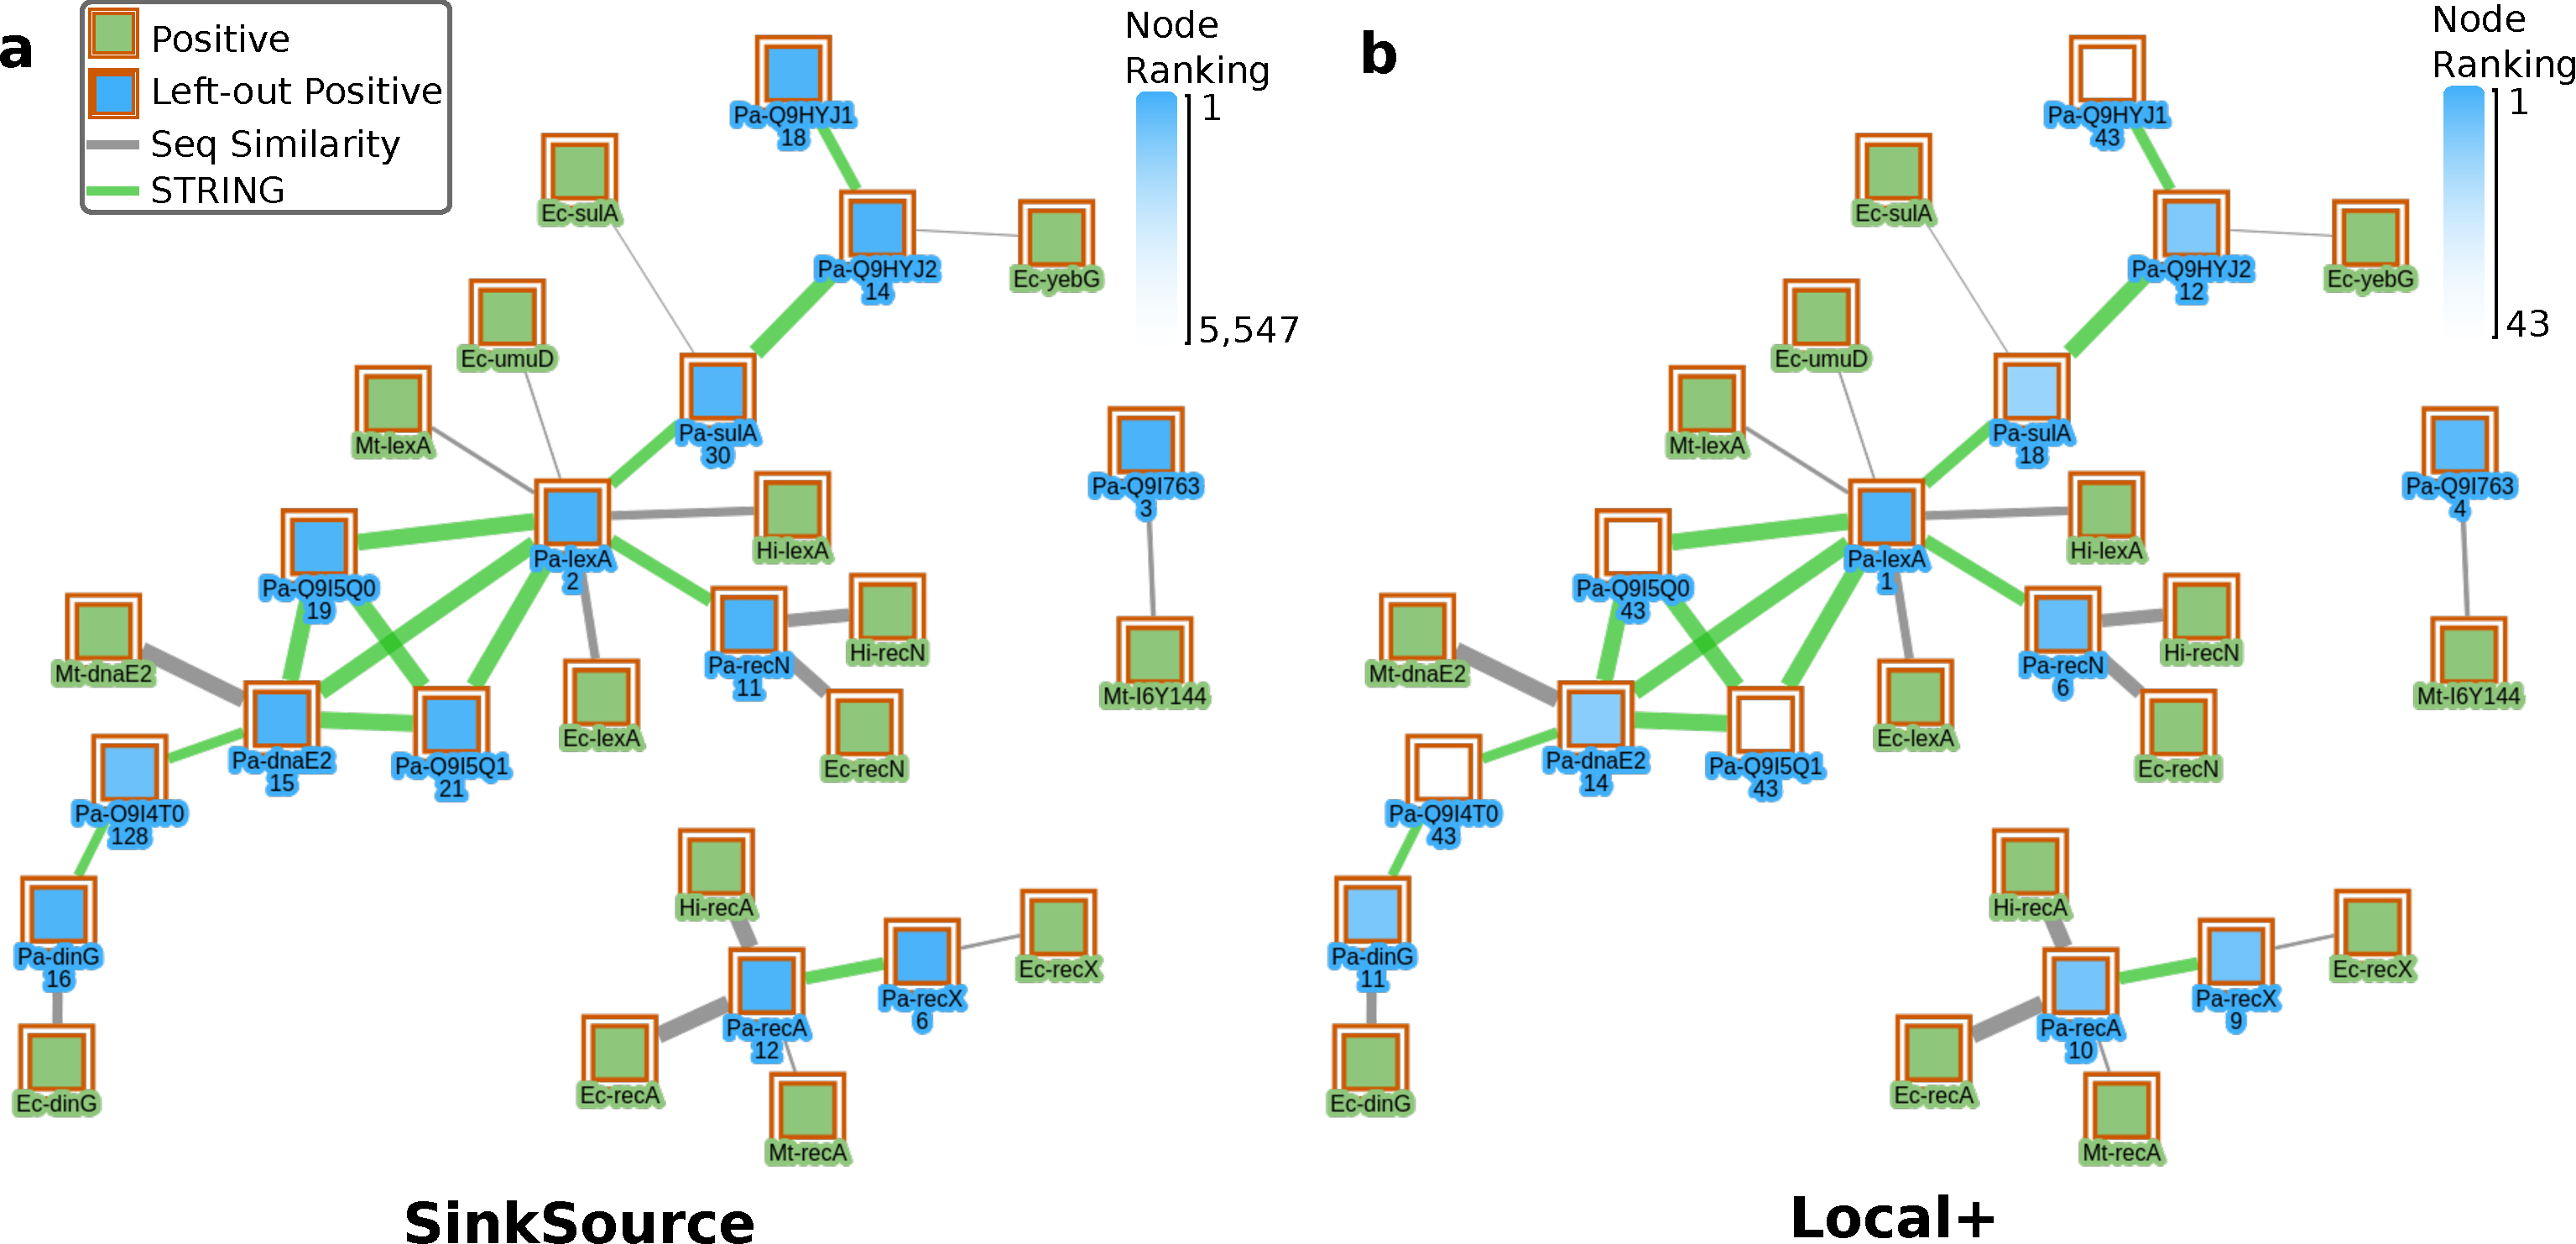
\includegraphics[width=\textwidth]{figs/fig4-sinksource-vs-localplus-sos-response.pdf}
    %\jeff{Add a scatterplot or something of the number of iterations and the median \fmax. Also add # of iterations and time taken}
    \caption{\sinksource comparison to \localplus. 
    Node rankings for left-out positives (blue) of \textit{P. aeruginosa} for example GO term "SOS response" GO:0009432. Nodes are colored by their rank.
    (a) \sinksource, (b) \localplus. \localplus is only able to give scores to 43 nodes, while \sinksource gives scores to almost all of the 5,575 \textit{P. aeruginosa} proteins.
    Species abbrev. same as in the caption of \cref{fig:loso-results-exp}.
    }
    \label{fig:sos-response-sinksource-vs-localplus}
\end{figure}


\begin{table}[htb]
    \centering
    \begin{tabular}{l|r|l}
    Method & Total Time (min) & Solver \\
    \hline
    \sinksource & 2.6  & 10 Iterations, $\alpha=0.95$ \\
    \genemania  & 44.0 & Conjugate Gradient ($tol=\e{-5}$) \\
    \birgrank   & 19.5 & Power Iteration ($\epsilon=\e{4}$) \\
    \localplus  & 0.3  & 1 Iteration \\
    \end{tabular}
    \caption{Total processor time of the four methods in minutes (\loso, BP terms, EXPC annotations) along with the type of solver used for each method. For \genemania, the reported time is the total process time used by CG across eight cores.}
    %\jeff{TODO times of weighting methods. SWSN: 6.4 min, indv GO terms 14.4 min (SS and \localplus), GM indv 39.9 min}
    \label{tab:loso-runtimes}
\end{table}


% EXPC + COMP, evaluate COMP
% EXPC + COMP + IEA, evaluate IEA
\subsection{LOSO Evaluation with Computational and Electronic Evidence Codes}
\label{sec:loso-results-expc-comp-iea}

\begin{figure}[H]
    \centering
    %\jeff{need to fix figure headings}
    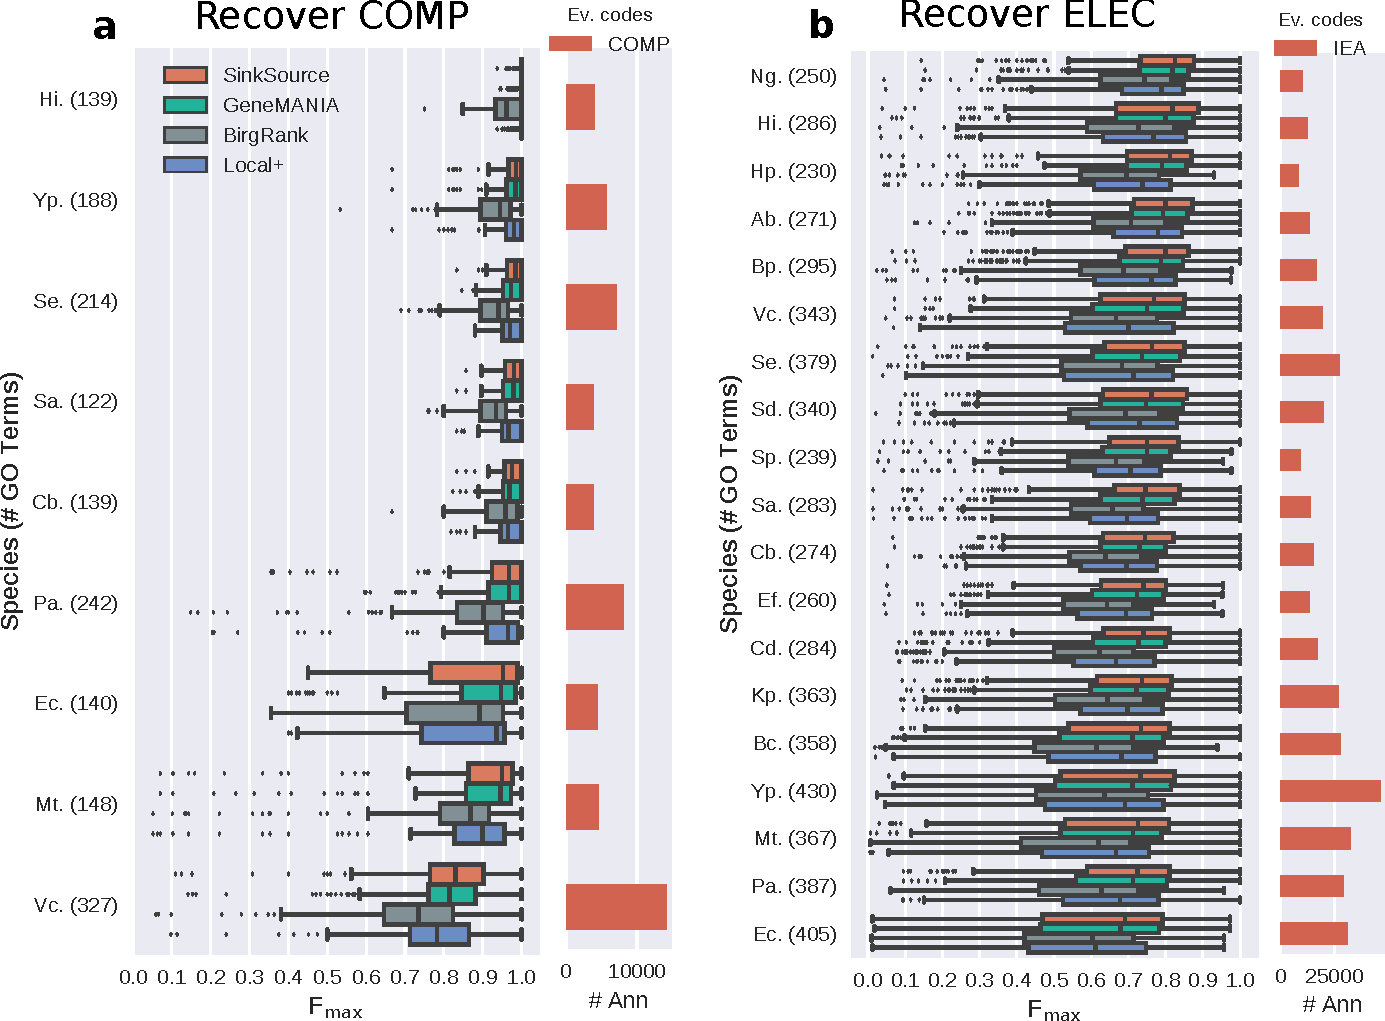
\includegraphics[width=\textwidth]{figs/fig3-expc-comp-iea.pdf}
    %\jeff{Add a scatterplot or something of the number of iterations and the median \fmax. Also add # of iterations and time taken}
    \caption{
      Comparison of \fmax results for the \loso evaluation for different evidence codes using the \SSN (\eval $\le$ 0.1) integrated with STRING. We made predictions using annotations with EXP and COMP evidence codes.
      (\textbf{a}) Evaluation of recovery of COMP evidence codes of the left-out species.
      (\textbf{b}) Evaluation of recovery of ELEC evidence codes (IEA) of the left-out species.
      Additional species names not defined in \cref{fig:loso-results-exp} are abbreviated as follows:
      \textit{Acinetobacter baumannii} (Ab), 
      \textit{Burkholderia cepacia} (Bc), 
      \textit{Bordetella pertussis} (Bp), 
      \textit{Clostridium botulinum} (Cb),
      \textit{Clostridioides difficile} (Cd), 
      \textit{Enterococcus faecium} (Ef),
      \textit{Haemophilus influenzae} (Hi),
      \textit{Helicobacter pylori} (Hp), 
      \textit{Klebsiella pneumoniae} (Kp),
      \textit{Staphylococcus aureus} (Sa),
      \textit{Shigella dysenteriae} (Sd),
      \textit{Streptococcus pyogenes} (Sp)
    }
    \label{fig:loso-results-expc-comp-iea}
\end{figure}

As most of our 19 organisms had little to no annotations based on experimental evidence (EXP), we expanded our analysis to include more organisms by mimicking the experimentally-based annotations with annotations based on computational analysis (COMP). 
%We evaluated and compare our methods using annotations with computational analysis evidence codes which are manually performed by a curator using sequence similarity (COMP), as well as automatic annotations with electronic evidence codes (ELEC). 
We repeated our \loso analysis using EXP and COMP annotations in 18 species, and evaluated each method's ability to recover the COMP annotations in the left-out species. A total of nine organisms had at least one BP GO term with 10 or more COMP annotations.

As expected, we immediately observed that recovering COMP annotations using a \SSN is much easier than recovering EXP annotations (see \cref{fig:loso-results-expc-comp-iea}a. For X/9 species, the improvement over \localplus was statistically significant.  

%\subsection{Temporal Holdout Evaluation}
%June 2016 - September 2017

\subsection{Scaling to 200 Bacterial Species}
\label{sec:loso-s200}

To test the ability of our methods to scale to include many more species, we built a \SSN with 200 bacterial species. 
%These species were chosen based on the criteria 
We chose the top 200 bacterial species with the most GO annotations with experimental and computational evidence codes. 
These species had a wide range of genome sizes varying from  protein-coding genes \jeff{TODO}. 
% 6,676 to 438 genes with at least one annotation (for \textit{Streptomyces bingchenggensis} NCBI:txid749414 and \textit{Mycoplasma genitalium} NCBI:txid243273 respectively) 
We also used an \eval cutoff of 0.1 for this \SSN, which yielded a network with 815K total proteins and 73M edges.
A total of 711 BP GO terms had 50 or more EXP or COMP annotations summed across the 200 species. 

We repeated the \loso evaluation with EXP and COMP annotations as in \cref{fig:loso-results-expc-comp-iea} with the 200 bacterial species where for each species in turn, we left-out all annotations for that species, then ran each algorithm with the EXP and COMP annotations to evaluate our ability to recover the left-out annotations. Rather than show the results for all 200 species individually, we summarized the results in \cref{tab:s200-loso-comp-iea}. 

We first observe the median \fmax of each algorithm are fairly similar to those in \cref{fig:loso-results-expc-comp-iea} and many of the observations made in that section remain true here. 
\jeff{Do the distributions for the 19-species increase?}
%Additionally, we find that 
% \jeff{Does the # of significant species increase? decrease? stay the same?}

\begin{table}[H]
    \centering
    \subfloat[Recover COMP]{
\begin{tabular}{|lccc|}
\hline 
Algorithm & Median  & MAD & \# Sig. Sp.\\
 & \fmax &  & (out of 42)\\
\hline
SinkSource & 0.984 & 0.02 & -\\
GeneMANIA & 0.984 & 0.02 & 0\\
BirgRank & 0.957 & 0.04 & 33\\
Local+ & 0.976 & 0.02 & 6\\
\hline 
\end{tabular}
    }
\quad
    \subfloat[Recover ELEC]{
\begin{tabular}{|lccc|}
\hline 
Algorithm & Median & MAD  & \# Sig. Sp.\\
 & \fmax  &  & (out of 200)\\
\hline
SinkSource & 0.750 & 0.09 & -\\
GeneMANIA & 0.756 & 0.10 & 0\\
BirgRank & 0.600 & 0.13 & 188\\
Local+ & 0.711 & 0.10 & 51\\
% with 20 iterations, 88 species are significant
\hline 
\end{tabular}
}

    \caption{
      Comparison of \fmax results of the \loso evaluation of different evidence codes using EXP and COMP annotations to make predictions for 200 bacterial species. MAD stands for Median Absolute Deviation. The column titled "\# Sig. Sp." shows the number of species for which the \fmax improvement of \sinksource over the given algorithm was statistically significant (rank-sum test, corrected by number of species)
      (\textbf{a}) Evaluation of recovery of COMP evidence codes of the left-out species. Total number of species - GO term pairs: 6,951.
      (\textbf{b}) Evaluation of recovery of ELEC evidence codes (IEA) of the left-out species. Total number of species - GO term pairs: 73,708.
}
    \label{tab:s200-loso-comp-iea}
\end{table}


% TODO include the total time in the previous table?
% \begin{table}[]
%     \centering
%     \begin{tabular}{c|c}
%          &  \\
%          & 
%     \end{tabular}
%     \caption{Total processor time of the four methods in hours}
%     \label{tab:my_label}
% \end{table}


\section{Discussion}

% Ripple: not going to include
% We also implemented the Ripple method for finding the top-k predictions for each GO term, but found that for GO terms with many annotations (50+) almost the entire network needed to be explored before the top-k could be ensured. For GO terms with less annotations, we found that the overhead associated with getting submatrices caused Ripple to take as long as runing regular sinksource.

\murali{Why use any more than three (Jeff says that with $\alpha=0.8$, even three iterations gives similar F-max distributions as 10 iterations or continuing till convergence) or 10 iterations (AptRank)? Why worry so much about making the intervals spanned by lower and upper bounds distinct? We have to thrash out this point.}

%\subsection{Scaling-up}


\bibliography{csb}
\bibliographystyle{unsrt}



%\input{network-based-pfp-pathogenic-bacteria-supp.tex}
% supplementary file for Accurate and Efficient Network-based Gene Function Prediction for Pathogenic Bacteria
%\documentclass{article}

%% Sets page size and margins
%\usepackage[margin=0.7in]{geometry}


\renewcommand{\thefigure}{S\arabic{figure}}
\renewcommand{\thetable}{S\arabic{table}}

\setcounter{figure}{0}
\clearpage
\appendix

% not sure how to make this an actual supplementary file
% appendix works for now 
%\title{Supplementary for Accurate and Efficient Network-based Gene Function Prediction for Pathogenic~Bacteria}
%\author[1]{Jeffrey N. Law}
%\author[2]{Shiv D. Kale}
%\author[3]{T. M. Murali}
%\affil[1]{Genetics, Bioinformatics, and Computational Biology Ph.D. program, Virginia~Tech, Blacksburg VA}
%\affil[2]{Biocomplexity Institute, Virginia Tech, Blacksburg VA}
%\affil[3]{Department of Computer Science, Virginia Tech, Blacksburg VA}
%%\affil[4]{ICTAS Center for Systems Biology of Engineered Tissues, Virginia Tech, Blacksburg VA}
%\date{September 2018}
%
%\maketitle

\section{Network Sizes}

Table \ref{tab:net-sizes} shows the number of nodes and edges for various BLAST \eval and STRING cutoffs.

\begin{table}[htb]
    \centering
\begin{tabular}{ccrr}
\SSN \eval & STRING &  & \\
cutoff & cutoff & \# Nodes & \# Edges \\
\hline
\e{-25} & - & 62,226 & 701,966\\
\e{-25} & 400 & 71,947 & 1,877,431\\
\e{-15} & - & 65,825 & 1,121,470\\
\e{-6} & - & 69,386 & 1,699,808\\
0.1 & - & 72,578 & 2,452,339\\
0.1 & 700 & 74,857 & 2,776,002\\
0.1 & 400 & 75,895 & 3,607,442\\
0.1 & 150 & 75,901 & 7,857,418\\
5 & - & 78,200 & 2,913,320\\
20 & - & 79,783 & 3,694,193\\
50 & - & 79,826 & 5,116,441\\
\end{tabular}
    \caption{Network sizes for various BLAST \eval and STRING cutoffs. }
    \label{tab:net-sizes}
\end{table}


\section{\birgrank results}
\label{sec:loso-birgrank}
\birgrank unfortunately did not perform as well as the other methods in our \loso evaluations. 
In the original evaluations of Jiang \textit{et al.}, they performed an evaluation where they whithheld all annotations from a given percentage of proteins and compared the ability of different algorithms to recover them. 
They observed that in this evaluation, their methods (\birgrank and AptRank) were not able to do better than \genemania and other methods. 
Our \loso evaluation seems to have exacerbated the problem for \birgrank. 
We varied the $\alpha$, $\theta$ and $\lambda$ parameters, but did not observe any improvement (results not shown).
\jeff{For five-fold cross-validation, \birgrank performed much better than \sinksource and \genemania (resuls not shown)}.

\section{MF Results}

\begin{figure}[H]
    \centering
    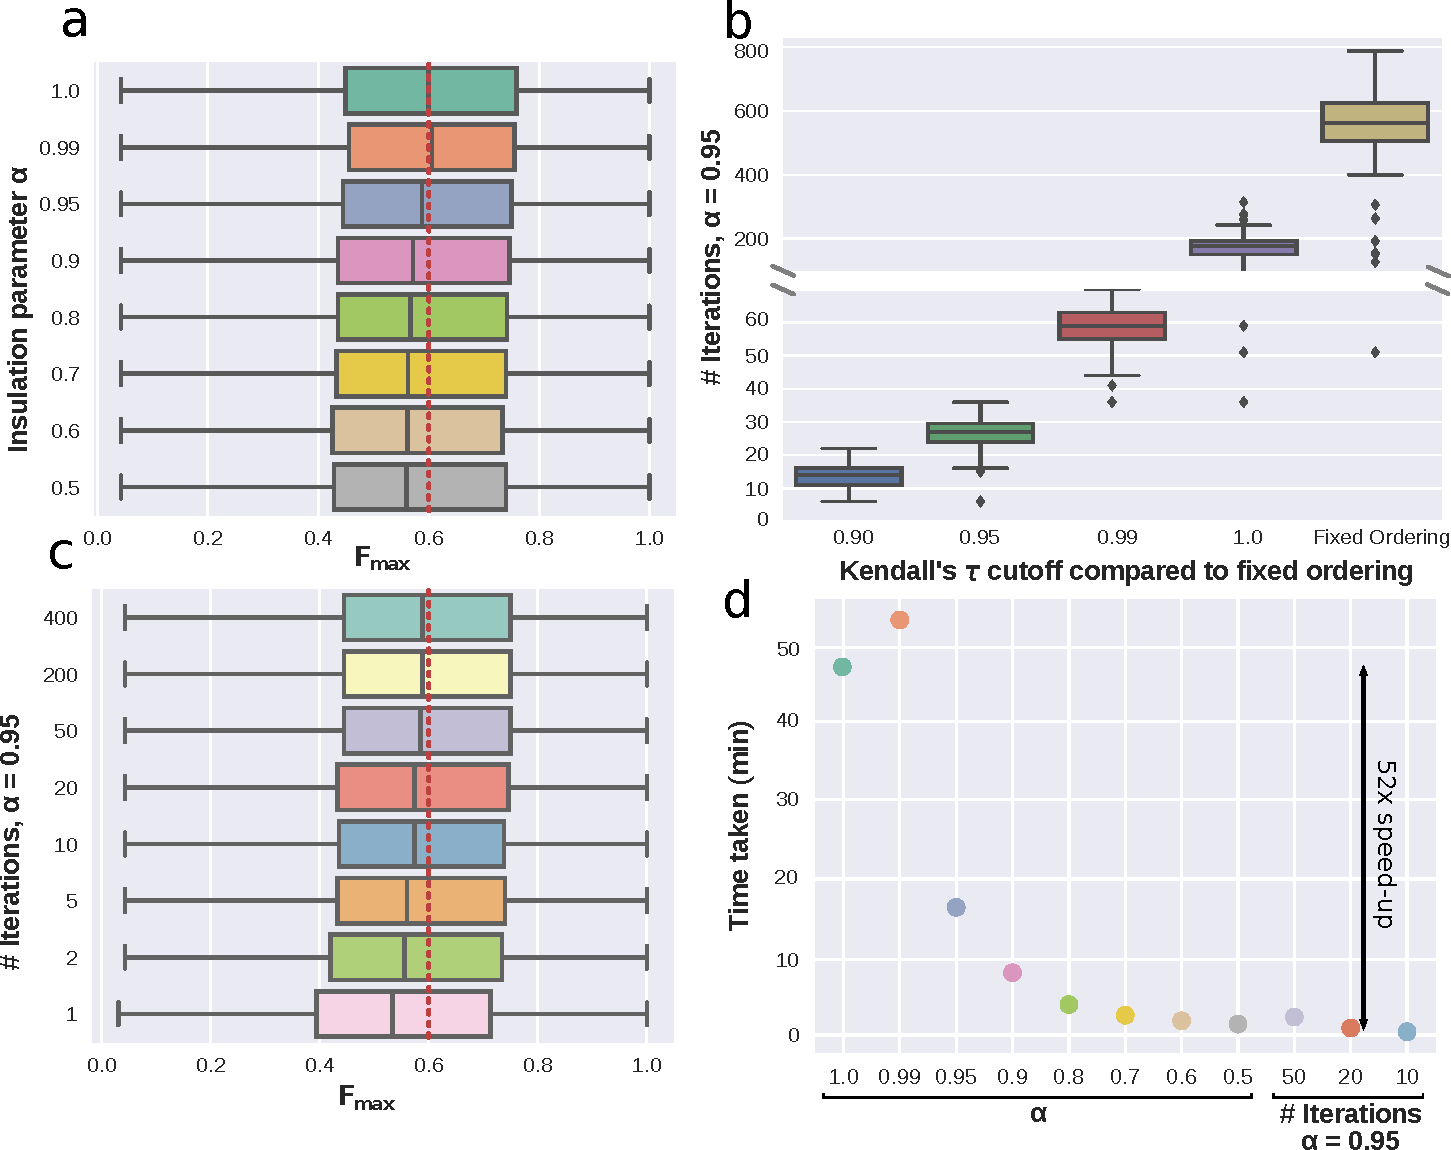
\includegraphics[width=\textwidth]{supp-figs/fig1-2018_06-seq-sim-e0_1-expc-rem-neg-comp-iea-50-1000-mf-a0_95.pdf}
    \caption{Trade-off between accuracy and speed for \sinksource on the 19 bacterial species \SSN (\eval <= 0.1) with 117 MF GO terms ($\ge 50$ annotations) for the \loso evaluation. 
      %Performance is measured by computing the \fmax on a GO term by GO term basis. Here we used annotations of BP GO terms with experimental evidence codes
      (\textbf{a}) Variation of \fmax distributions with $\alpha$. The vertical red dotted line represents the median \fmax for $\alpha = 1.0$.
      (\textbf{b}) Number of iterations required to fix the rankings of the left-out positives and negatives, or to reach a specified value of \ktau in comparison to the fixed ranking.
      (\textbf{c}) Variation of \fmax distributions with the number of iterations ($\alpha=0.95$). The vertical red dotted line represents the median \fmax for $\alpha = 1.0$ in panel (a).
      (\textbf{d}) Total time taken by \sinksource (shown in a and b) while varying $\alpha$ or the number of iterations with $\alpha=0.95$. Colors are the same as in (\textbf{a}) and (\textbf{c}).
    }
    \label{fig:sinksource-speed-vs-accuracy-mf}
\end{figure}


%\jeff{MF SinkSource increase from e1e-25 to e0_1 rank-sum test \pval $2.6\times{}10^{-7}$ )}
\begin{figure}[H]
    \centering
    %\jeff{figure placeholder}
    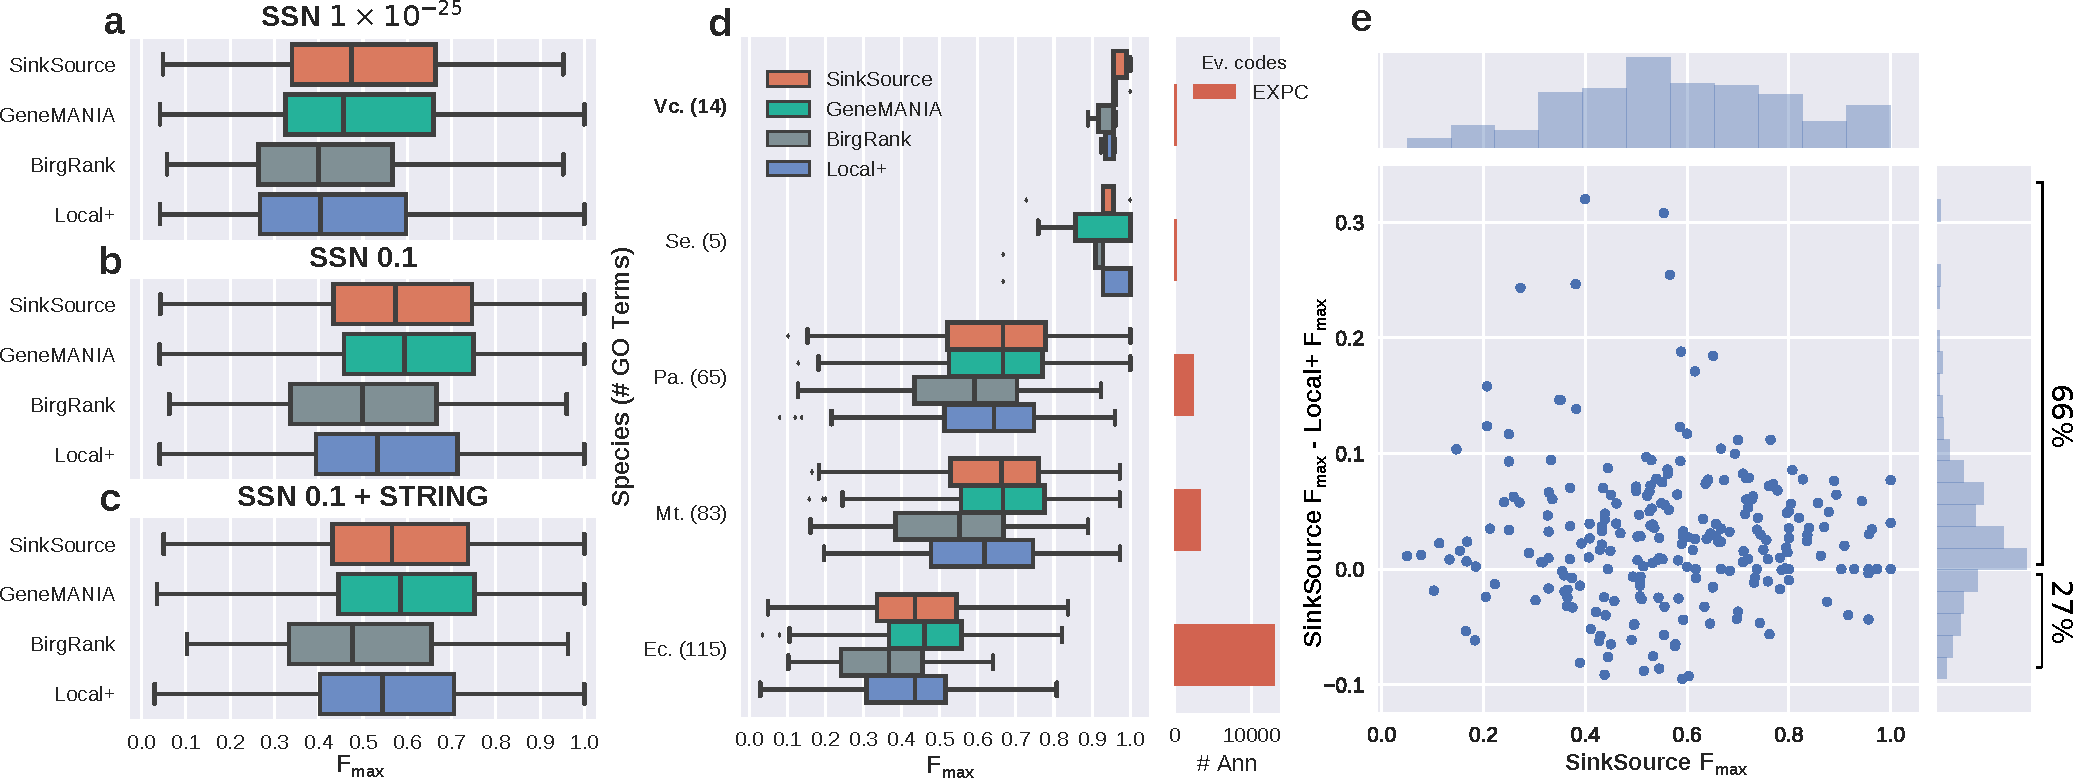
\includegraphics[width=\textwidth]{supp-figs/fig2-expc-compare-eval-fmax-sinksource-localplus-mf-a0_95.pdf}
    \caption{
      Comparison of \fmax results for \loso evaluation of four algorithms and three networks.
      (\textbf{a}) \SSN (\eval $\le$ \e{-25}),
      (\textbf{b}) \SSN (\eval $\le$ 0.1),
      (\textbf{c},\textbf{d},\textbf{e}) \SSN (\eval $\le$ 0.1) integrated with STRING,
      (\textbf{d}) \loso results for individual species, sorted in decreasing order of median \fmax. The number of MF GO terms with $\ge$ 10 annotations appears in parentheses next to each species name.  The species name is in bold if the difference between the distributions for \sinksource and \localplus was statistically significant (rank-sum Bonferroni-corrected \pval $< 0.05$). \protect The right-hand side shows the number of GO term-annotation pairs with experimental evidence codes for each species.
    %315 total BP GO terms have at least 10 annotations in the left-out species. 
    Species names are abbreviated as follows:
    \textit{Escherichia coli K-12} (Ec),
    \textit{Mycobacterium tuberculosis} (Mt),
    \textit{Neisseria gonorrhoeae} (Ng),
    \textit{Pseudomonas aeruginosa} (Pa),
    \textit{Salmonella enterica} (Se),
    \textit{Vibrio cholerae} (Vc),
    \textit{Yersinia pestis} (Yp).
    (\textbf{e}) Difference in \fmax between \sinksource and \localplus by the \fmax of \sinksource for each GO term. 
    %Comparison of using a \SSN with a cutoff of $1\times{}10^{-25}$ vs. a cutoff of $0.1$. The \fmax results for each individual species are combined and shown in a single box-plot for each algorithm.}
    }
    \label{fig:loso-results-exp-mf}
\end{figure}


\begin{figure} 
    \centering
    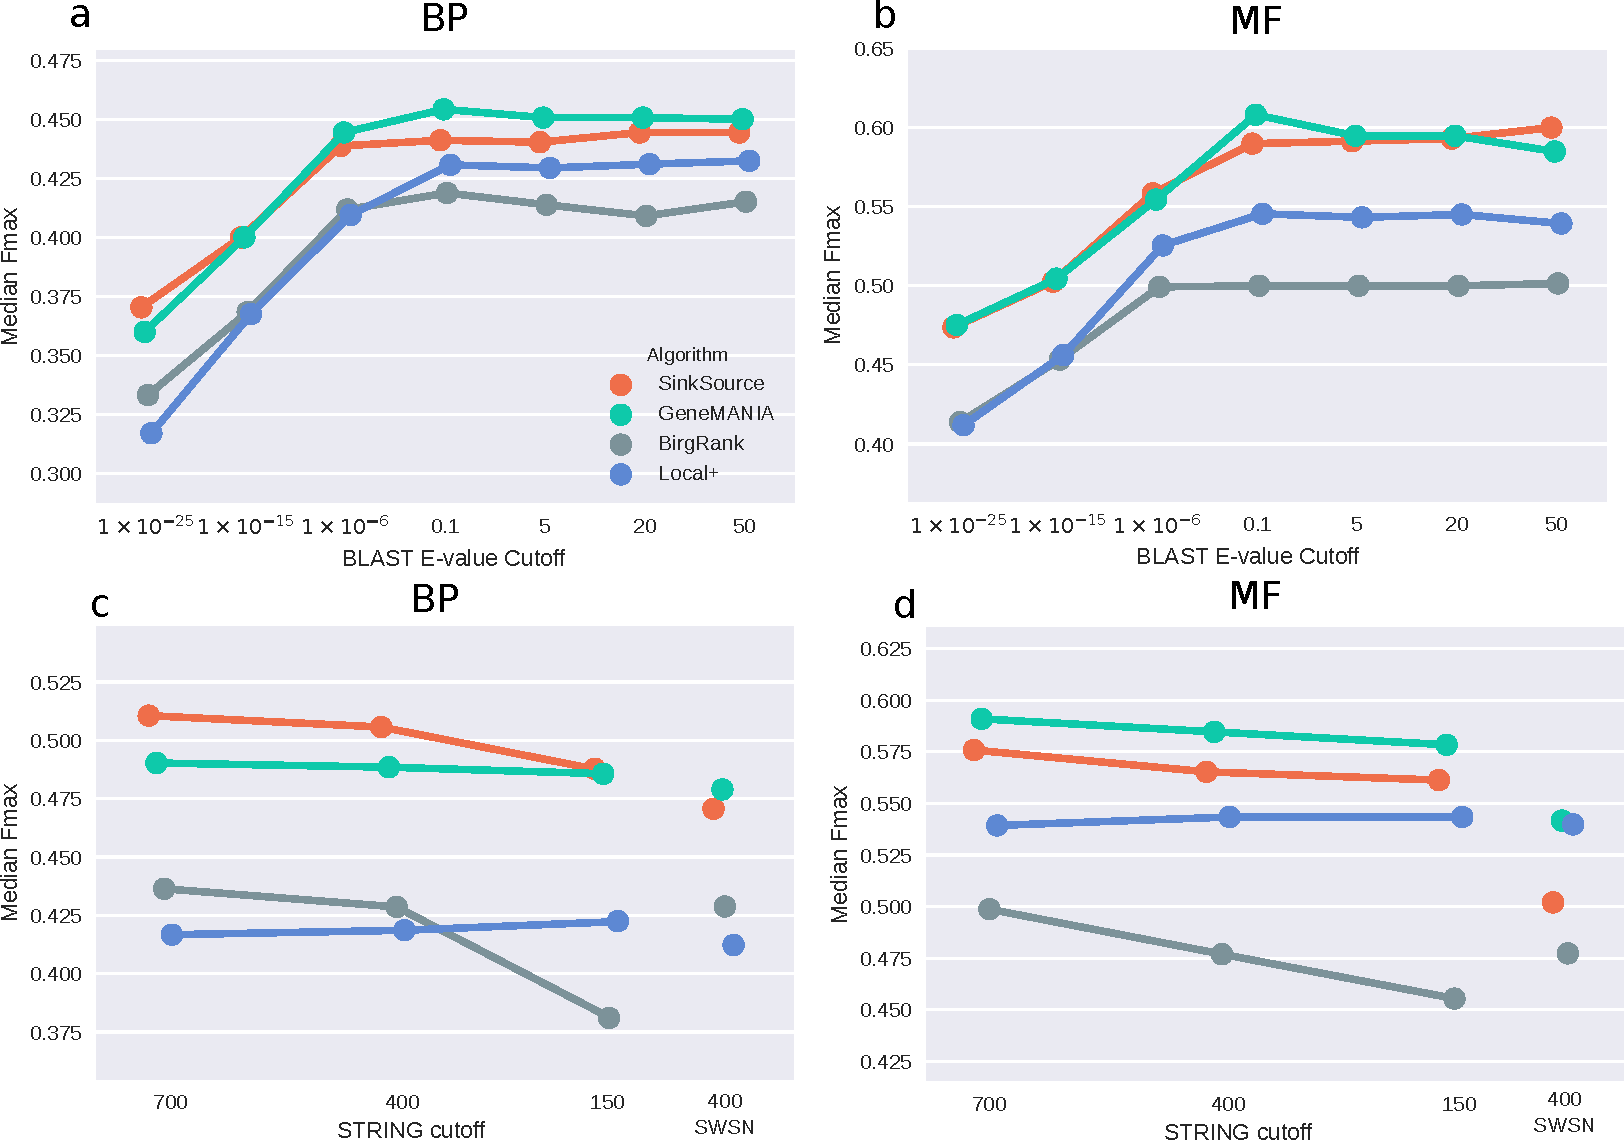
\includegraphics[width=\textwidth]{supp-figs/compare-eval-string-cutoffs-fmax-nobars.pdf}
    \caption{Comparison of \fmax results for \loso evaluation of EXPC annotations using various BLAST E-value cutoffs (\textbf{a}, \textbf{b}) and STRING cutoffs (\textbf{c}, \textbf{d}).
    For each algorithm and network, the plot shows the median \fmax as well as the 95\% confidence interval of the median using 1000 bootstrap samples.
    The last column of the \textbf{c} and \textbf{d} shows the results when using the SWSN method to weight the network with a STRING cutoff of 400.
    }
    \label{sfig:compare-eval-string-cutoffs}
\end{figure}


\begin{figure}
    \centering
    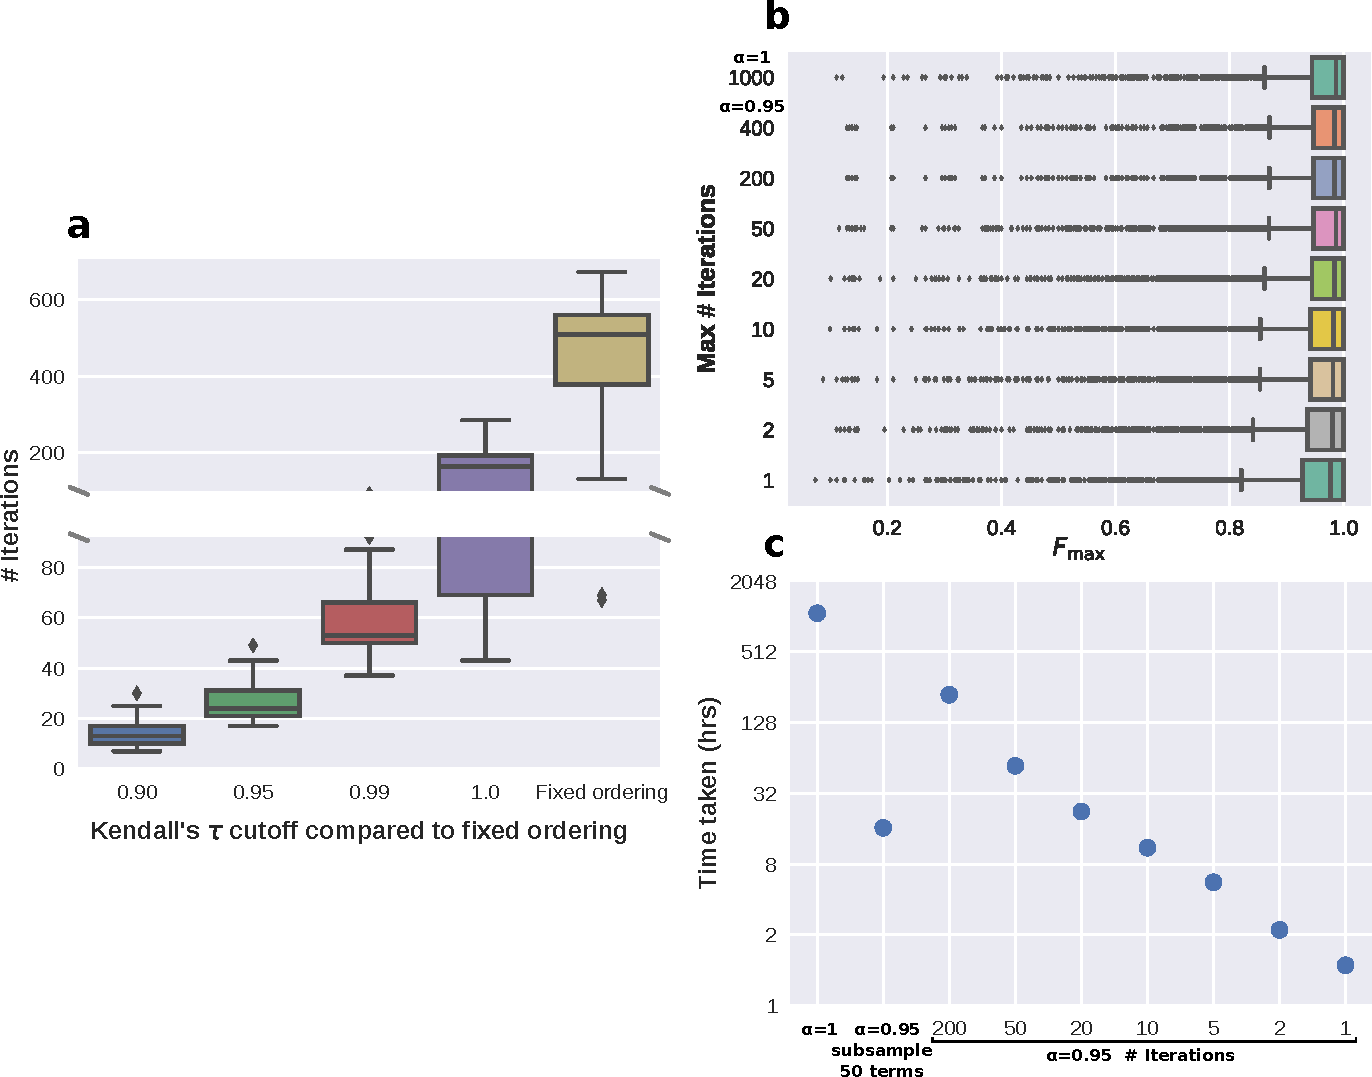
\includegraphics[width=\textwidth]{supp-figs/fig1-s200-expc-comp-rem-neg-iea-comp-bp-a0_95.pdf}
    \caption{Trade-off between accuracy and speed for SinkSource on the 200 bacterial species SSN (\eval $\leq$ 0.1) with 511 BP GO terms ($\geq 50$ annotations) for the LOSO evaluation using EXPC and COMP to make predictions, and COMP to evaluate in the left-out species.}
    \label{fig:my_label}
\end{figure}


\begin{figure}[H]
    \centering
    %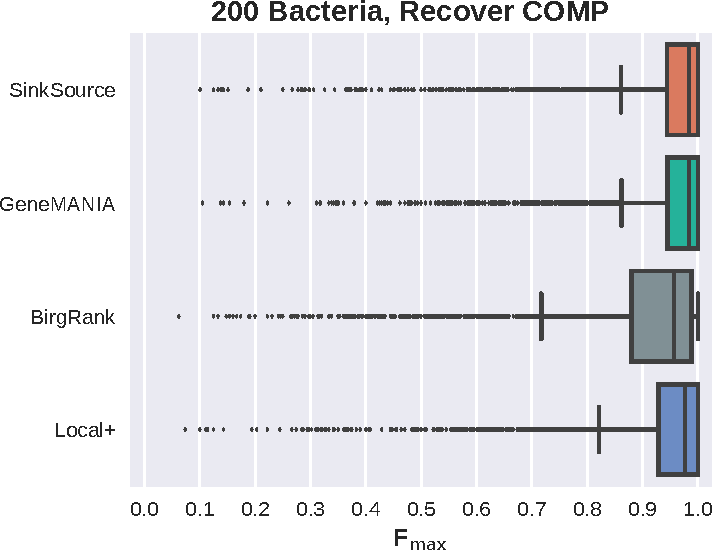
\includegraphics[width=\textwidth]{figs/s200-expc-comp-recover-comp-bp-4-use-neg-fmax-boxplot.pdf}
    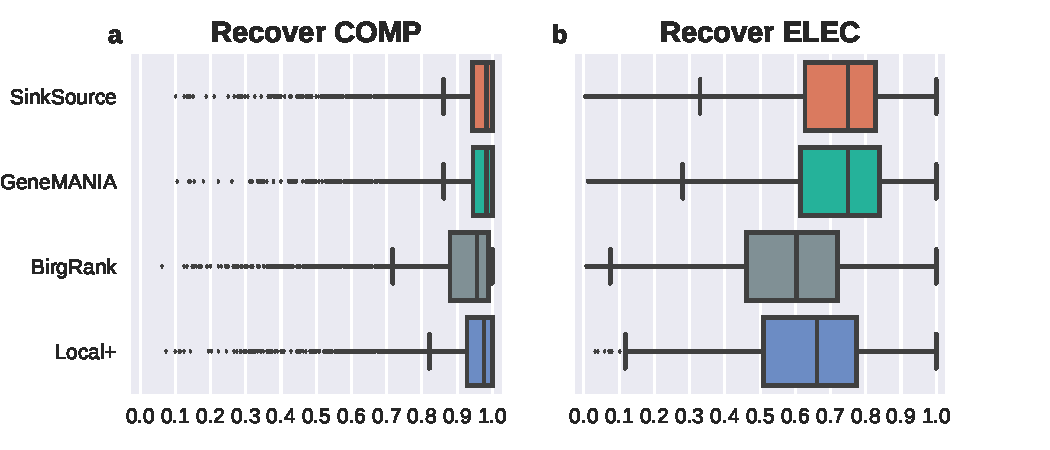
\includegraphics[width=\textwidth]{figs/s200-eval-comp-iea-fmax-boxplots-bp-0_95.pdf}
    \caption{
      Comparison of \fmax results of the \loso evaluation of different evidence codes using EXP and COMP annotations to make predictions for 200 bacterial species. 
      (\textbf{a}) Evaluation of recovery of COMP evidence codes of the left-out species.
      (\textbf{b}) Evaluation of recovery of ELEC evidence codes (IEA) of the left-out species.
    }
    \label{fig:s200-loso-results-expc-comp}
\end{figure}


\end{document}
